\documentclass[12pt,a4paper]{article}
\usepackage{graphicx}
\usepackage{amsmath}
\usepackage{mathtools}
\usepackage[T1]{fontenc}
\usepackage{charter}
%\usepackage{subfig}
%\usepackage{color,soul}
\usepackage{xcolor}
\usepackage{indentfirst}
\usepackage[colorlinks,linkcolor=black,urlcolor=blue,citecolor=blue]{hyperref}
\usepackage[numbers]{natbib}
\usepackage{doi}
\usepackage{xpatch}
\usepackage[left=2.0cm, right=2.0cm, top=2cm, bottom=2cm]{geometry}
\usepackage[font=small,labelfont=bf]{caption}
\usepackage{subcaption}
\usepackage{parskip}
\usepackage{setspace}

\setlength{\parskip}{5pt}
\onehalfspacing

\begin{document}
\begin{titlepage}
\title{Modulation Instability in Semiconductor Quantum Dots\\[0.2em]
    \textit{(Y-type Excitation Scheme)}}
\author{
    \textit{Submitted by,}\\
    {Shaon Samanta}\\
    {SEM-III, Department of Physics, Roll No. 38, RKMVCC}\\[3ex]
    {Under the supervision of,}\\
    {Dr. Rohit Mukherjee}\\
    {Assistant Professor, Department of Physics, Sarala Birla University}
}

\makeatletter         
\def\@maketitle{
\begin{center}
\vspace*{1.5cm}
{\Huge \bfseries \@title}\\[5.5ex]

\includegraphics[width=80mm]{pictures/rkmlogo.png}\\[4ex]
{\LARGE  \@author}\\[4ex] 
%\@date\\[8ex]
\end{center}}
\makeatother

\maketitle
\thispagestyle{empty}
\end{titlepage}

\tableofcontents
\pagebreak

\begin{abstract}
    This study explores the phenomenon of modulation instability (MI) within semiconductor quantum dots (SQDs), emphasizing its implications for nonlinear optics and quantum information technologies. MI, which is defined as the exponential amplification of perturbations in nonlinear dispersive media, is studied in the context of SQDs due to their unique quantum confinement effects, which lead to enhanced optical nonlinearities. The research creates a mathematical model that uses density matrix formalism and nonlinear Schrödinger equations to analyze MI-induced dynamics. This framework facilitates a deeper understanding of light-matter interactions, which is critical for advancing applications in quantum computing, secure communication, and high-efficiency optical devices. The findings contribute to the optimization of SQD-based systems, highlighting their potential in next-generation photonic and quantum technology.
\end{abstract}

\section{Introduction}
Since the advent of working example of photonic crystal fibers (PCFs) in 1996~\cite{photoniccrystal}, MI study has geared up in these media extensively, taken into account the flexibility to adjust the dispersion profile. Though initially, the MI was studied in anomalous dispersion regime, but in 2003 Harvey et al.\cite{harvey2003scalar} have demonstrated the role of MI in the normal dispersion regime also.\par
Studies and experiments on MI have started almost simultaneously across the world around 1965's. The earlier approach to solving MI follows the classical Lighthill criterion~\cite{lighthall}, which is considered when nonlinearity and dispersion make opposite contribution to wave frequency. Numerous investigations on wave instability in optical fibers reveal wave mixing instabilities that are not addressed by the Lighthill criterion~\cite{lighthall}, were solved using generalized nonlinear Schr\"{o}dinger equation (NLSE)~\cite{RBoyd}. Unstable propagation of continuous (CW) or quasi-continuous waves (QCW) in nonlinear media possessing Kerr nonlinearity and higher-order dispersion is found to be responsible for generation of spectral sidebands.

\section{Semiconductor Quantum Dots (SQDs)}
Semiconductor quantum dots are tiny particles or nanocrystals of a semiconducting material with diameters in the range of 2-10 nanometers (10-50 atoms). They were first discovered in 1980~\cite{quantumdots1980}. They display unique electronic properties, intermediate between those of bulk semiconductors and discrete molecules [See Figure 1], that are partly the result of the unusually high surface-to-volume ratios for these particles. The most apparent result of this is fluorescence, wherein the nanocrystals can produce distinctive colors determined by the size of the particles.

\begin{figure}[h]
    \centering
    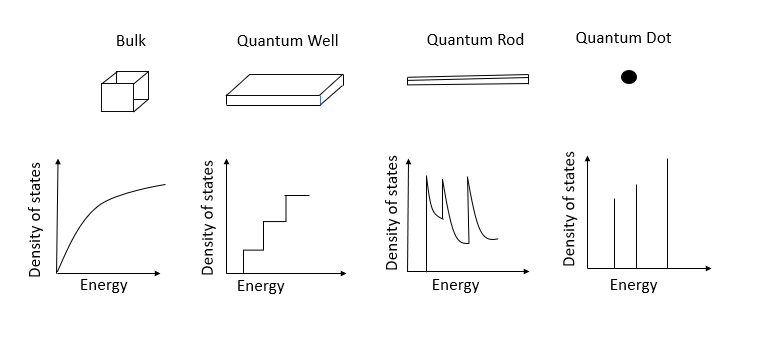
\includegraphics[width=0.6\linewidth]{./pictures/DoSvsE.png}
    \caption{Density of states vs energy of materials}
    \label{fig:DoS vs Energy of materials}
\end{figure}

\subsection{Quantum Coherence and Interference}
Quantum Coherence refers to the property of quantum systems where particles exist in a superposition of states, which allow the interference of quantum waves~\cite{Scully_Zubairy_1997}. Coherence is essential for the occurrence of quantum interference, which is the interaction between these superposed states. It is fundamental in quantum phenomena like entanglement, superposition, and wave-particle duality. It enables systems to maintain phase relationships between quantum states, which is critical for processes like constructive and destructive interference in both matter and light waves.\par
Quantum interference is a phenomenon when subatomic particles interact with and influence themselves and other particles while in a probabilistic superposition state~\cite{Scully_Zubairy_1997}. When a particle is in a superposition of multiple states, these states can interfere with each other leading to constructive or destructive interference. Quantum interference, along with quantum entanglement, is essential to the operation of quantum computers.

\section{Origin of Non-linear Optics}
Nonlinear optics is the study of phenomena that occurs as a consequence of the modifying the optical properties of a material system by the usage of light. Basically,only laser light is sufficiently intense to modify the optical properties of a material system in the manner.The beginning of the field of nonlinear optics is often taken to be the discovery of second-harmonic generation by Franken et al.~\cite{PhysRevLett.7.118} (1961), shortly after the demonstration of the first working laser by Maiman in 1960~\cite{laserdev}. Nonlinear optical phenomena are “nonlinear” in the sense that they occur when the response of a material system to an applied optical field depends in a nonlinear manner on the strength of the applied optical field.The field of nonlinear optics is now sixty three tears old.Interest in this field has grown continuously since it's beginnings,and the field of nonlinear optics now ranges from fundamental studies of the interaction of light with matter~\cite{lightmatter2022} to applications such as laser frequency conversion and
optical switching.

\section{Modulation Instability (MI)}
Modulation instability or sideband instability is a phenomenon whereby deviations from a periodic waveform are reinforced by nonlinearity, leading to the generation of spectral-sidebands and the eventual breakup of the waveform into a train of pulses.\par
MI has received special attention in optical fibers, since they possess high nonlinearity and tailorable dispersion profile. The first experimental observation of MI effect was reported by Tai et al. in 1986~\cite{tai1986generation}. Extension of MI to the normal dispersion regime was predicted in 1970. Since, then numerous researches were exerted towards improvement of MI spectra. A decade back, Erkintalo et al.~\cite{erkintalo2011higher} have reported a theoretical and experimental study on higher order MI in optical fibers. MI in dispersion oscillating fibers has reported by Mussot et al.~\cite{mussot2017modulation}. Recently, Kraych~\cite{kraych2019nonlinear} have reported a unique behavior in the evolution of a modulationally unstable plane wave driven by a small noise in fiber optics. In a recent study, Liu et al.~\cite{liu2021exact} have reported to obtain asymmetric spectra of MI by applying asymmetric physical effect called self-steepening.\par
It is widely believed that the phenomenon was first discovered and modeled for periodic surface gravity waves (Stokes waves) on deep water by T. Brooke Benjamin and Jim E. Feir~\cite{Benjamin_Feir_1967}, in 1967. Therefore, it is also known as the Benjamin-Feir instability. Modulation instability (MI) is a fundamental phenomenon associated with an exponential growth of weak perturbed waves, during their propagation through nonlinear dispersive media. It occurs due to the interaction of nonlinear and dispersive effects which lead to the disintegration of waves into a train of shape preserving ultrashort pulses~\cite{MANUKURE2021100140}.\par
Semiconductor quantum dots exhibit strong nonlinearities~\cite{Scully_Zubairy_1997} due to quantum confinement effects, leading to larger optical susceptibilities. Modulation instability, as a manifestation of nonlinear effects, provides insight into how these nonlinearities can amplify perturbations in the system, which is critical for optimizing optical device performance.\par
Understanding Modulation Instability is relevant for quantum information technologies like quantum computers. Modulation Instability can impact entanglement generation, quantum coherence, and light-matter interaction dynamics, which are essential for quantum computing and secure communication.

\section{Mathematical Model}
\begin{figure}[h]
    \centering
    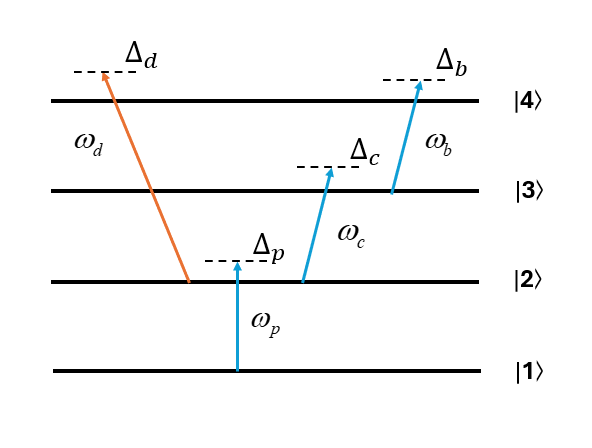
\includegraphics[width=0.6\linewidth]{pictures/Y-type.png}
    \caption{Y-type excitation scheme arrangement of GaAs quantum dots under study.}
    \label{fig:Y-type Excitation Scheme}
\end{figure}

This is a four-level Y-type excitation scheme with \(E_1,E_2,E_3,E_4\) energies of GaAs quantum dots. The quantum dots system interacts with one continuous wave (CW) or quasicontinuous probe field of amplitude \(E_p\) with angular frequency \(\omega_p\) and two control laser field \(E_c\) and \(E_b\) with angular frequencies \(\omega_c\) and \(\omega_b\) respectively. There is a coupling field \(E_d\) between energy level \(|2\rangle\) and \(|4\rangle\) with angular frequency \(\omega_d\). The probe field acts on the transition from \(|1\rangle\) to \(|2\rangle\), while the two control fields act on the transitions from \(|2\rangle\) to \(|3\rangle\), \(|3\rangle\) to \(|4\rangle\) respectively and coupling field from \(|2\rangle\) to \(|4\rangle\). All the lights propagate along the \(z\)-axis within the QD sample.\\
 The electric fields interacting inside the QD can be written as:
 \begin{equation}
     \vec{E}=\sum_{j=p,c,b}\hat{e_j}E_j e^{i(k_j z-\omega_j t)}+c.c.
 \end{equation}
where \(\hat{e_j}\) are the unit vectors along the polarization direction of the probe and control fields, \(k_j\) is the wave vector of the applied field, and the subscripts \(p,\ c,\ b\) and \(d\) signify the probe, first, second control fields and coupling fields respectively. The term \(c.c\). refers to the complex conjugate.\par
Adopting the rotating wave approximation (RWA) the semiclassical Hamiltonian of the coupled quantum well system can be written as:
\begin{equation}
    \hat{H}=\hat{H}_0+\hat{H}_{int},
\end{equation}
where,
\begin{equation}
    \hat{H}_0=\sum_{j=1}^4E_j|j\rangle\langle j|,
\end{equation}
and,
\begin{align}
    \hat{H}_{int} = -\hbar[\Omega_p e^{i(k_p z-\omega_p t)}|2\rangle\langle 1|+\Omega_c e^{i(k_c z-\omega_c t)}|3\rangle\langle 2|&+\Omega_b e^{i(k_b z-\omega_b t)}|4\rangle\langle 3|\nonumber\\&+\Omega_d e^{i(k_d z-\omega_d t)}|4\rangle\langle 2|+H.c.].
\end{align}.
Here, \(\hat{H}_0\) represents the unperturbed Hamiltonian of the system in the absence of applied fields, and \(\hat{H}_{int}\) describes the interaction of the electrons in the semiconductor quantum dots with the electromagnetic fields. Due to the closed-loop configuration, the properties of the SQDs are quite sensitive to the phases of the applied fields. These phases are incorporated into the inter-subband transition Rabi frequencies of the probe \((\Omega_p)\), control fields \(\Omega_c\), \(\Omega_b\) and coupling field \(\Omega_d\) defined as:
\begin{align}
    \Omega_p &=|\Omega_p|=\frac{\mu_{21}\hat{e}_p E_p}{\hbar},\\
    \Omega_c &=|\Omega_c|=\frac{\mu_{32}\hat{e}_c E_c}{\hbar},\\
    \Omega_b &=|\Omega_b|=\frac{\mu_{43}\hat{e}_b E_b}{\hbar},\\
    \Omega_d &=|\Omega_d|=\frac{\mu_{42}\hat{e}_d E_d}{\hbar},
\end{align}
here, \(\mu_{mn}=e\langle m|\hat{z}|n\rangle\) is the electronic dipole moment matrix element between transitions \(|m\rangle\leftrightarrow |n\rangle\).

\subsection{Density Matrix Formalism}
To study the light-matter interaction phenomena occurring in the QD system, we use the density matrix formalism \cite{BOYD2008135}:
\begin{equation}
    \frac{\partial \rho_{ij}}{\partial t} = -\frac{i}{\hbar} \sum_m \left( H_{im} \rho_{mj} - \rho_{im} H_{mj} \right) - \frac{1}{2} \left( \Gamma_{im} \rho_{mj} + \rho_{im} \Gamma_{mj} \right),
\end{equation}
where \(\rho_{ij}\) is the \(ij^{\text{th}}\) density matrix element. The first term on the right-hand side represents the coherent evolution of the state, while the second term represents radiative decay processes. The decay matrix \(\Gamma\) is defined as:
\begin{equation}
    \Gamma_{im} = \langle i|\Gamma|m\rangle = \gamma_i\delta_{im},
\end{equation}
where $\gamma_i$ represents the population decay rate of the $i^{\text{th}}$ energy level.

So from the Maxwell's Bloch equation for the density matrix elements we can write:
\begin{equation}
    \frac{\partial\tilde\rho_{21}}{\partial t} = i\big(\Delta_p+i\frac{\gamma_{21}}{2}\big)\tilde{\rho}_{21}+i\Omega_c^*\tilde{\rho}_{31}+i\Omega_d^*\tilde{\rho}_{41}+i\big(\tilde{\rho}_{11}-\tilde{\rho}_{22}\big)\Omega_p,
\end{equation}
\begin{equation}
    \frac{\partial\tilde{\rho}_{31}}{\partial t}=i\big(\Delta_p+\Delta_c+i\frac{\gamma_{31}}{2}\big)\tilde{\rho}_{31}+i\Omega_c\tilde{\rho}_{21}+i\Omega_d^*\tilde{\rho}_{41}-i\Omega_p\tilde{\rho}_{34},
\end{equation}
\begin{equation}
    \frac{\partial\tilde{\rho}_{41}}{\partial t}=i\big(\Delta_p+\Delta_d+i\frac{\gamma_{41}}{2}\big)\tilde{\rho}_{41}+i\Omega_d\tilde{\rho}_{21}+i\Omega_b\tilde{\rho}_{31}-i\tilde{\rho}_{42}\Omega_p,
\end{equation}
where $\Delta_j{(j=p,\ c,\ b,\ d)}$ is the detuning frequency of the corresponding applied field, which is defined as:
\begin{align}
\Delta_p &= \omega_{p}-\frac{E_2-E_1}{\hbar},\\
\Delta_c &= \omega_{c}-\frac{E_3-E_2}{\hbar},\\
\Delta_d &= \omega_{d}-\frac{E_4-E_2}{\hbar},\\
\Delta_b &= \omega_{b}-\frac{E_4-E_3}{\hbar},
\end{align}
respectively. The population conservation condition \(\sum_{i=1}^{4} \tilde\rho_{ii} = 1\), together with $\rho_{mj} = \rho_{jm}^*{(m,\ j=1,2,3,4)}$ ${(;m\neq j)}$, supplements the above equation. Moreover, we have used the following transformations:
\begin{align}
    \rho_{21} &= \tilde\rho_{21}e^{-i(k_p z-\omega_p t)},\\
    \rho_{31} &= \tilde\rho_{31}e^{i(k_p z-\omega_p t)}e^{-i(k_c z-\omega_c t)},\\
    \rho_{41} &= \tilde\rho_{41}e^{-i(k_p z-\omega_p t)}e^{-i(k_d z-\omega_d t)},\\
    \rho_{32} &= \tilde\rho_{32}e^{-i(k_c z-\omega_c t)},\\
    \rho_{43} &= \tilde\rho_{43}e^{-i(k_b z-\omega_b t)},
\end{align}.
In semiconductor QDs, $\gamma_{jl} = \gamma^{dph}_{jl}{(j=2-4)}$ signifies that total population decay rate from the energy subband $|j\rangle$, which cocsists of a population decay rate  due to inelastic "Low Order" phonon emission at low temperature and a dephasing term $\left(\gamma^{dph}_{jl}\right)$ originates not only from electron-electron and electron-proton scattering.\par
In the steady state we assume that all the electrons will initially occupy the ground state that is,i.e., $\tilde\rho_{11} = 1, \tilde\rho_{ii}{(i=2,3,4)}=0$ at t=0. Under the limit of weak probe field approximation, we may also assume that probe field also sufficiently weak in comparison to control fields[i.e., $\Omega_p \ll \Omega_c,\Omega_b$; Therefore we will introduce the perturbative expansion $\tilde\rho_{ij} = \sum\limits_{k} \tilde\rho^{(k)}_{ij}$, where $\tilde\rho^{(k)}_{ij}$ is the \(k^{\text{th}}\)-order perturbation of ${\tilde\rho}_{ij}$. From the regime of adibatic formulation,it can be easily shown that ${{\tilde\rho}^{(0)}}_{ij}=\delta_{ij}(i\neq j)$, ${{\tilde\rho}^{(0)}}_{ii}(i=2,3,4)\simeq0$,and$\tilde\rho_{j1}\simeq{{\tilde\rho}^{(1)}}_{j1}{{\tilde\rho}^{(0)}}_{11}$ (j=2,3,4).Note that $\tilde\rho_{11}$ is the population density matrix element,while $\tilde\rho_{ij}$ is the optical response to the probe field for transition $|i\rangle$ $\rightarrow$ $|j\rangle$.Therefore the population conservation condition is valid for the zeroth order in the perturbative expansion and not valid for higher order terms, i.e., \({{\tilde\rho}^{(0)}}_{11}+{{\tilde\rho}^{(0)}}_{22}+{{\tilde\rho}^{(0)}}_{33}+{{\tilde\rho}^{(0)}}_{44}=1\). So equations- (11)-(13) reduces to:
\begin{equation}
    \frac{\partial\tilde\rho_{21}^{(1)}}{\partial t} = i\big(\Delta_p+i\frac{\gamma_{21}}{2}\big)\tilde{\rho}_{21}^{(1)}+i\Omega_c^*\tilde{\rho}_{31}^{(1)}+i\Omega_d^*\tilde{\rho}_{41}^{(1)}+i\big(\tilde{\rho}_{11}^{(0)}-\tilde{\rho}_{22}^{(0)}\big)\Omega_p,
\end{equation}
\begin{equation}
    \frac{\partial\tilde{\rho}_{31}^{(1)}}{\partial t}=i\big(\Delta_p+\Delta_c+i\frac{\gamma_{31}}{2}\big)\tilde{\rho}_{31}^{(1)}+i\Omega_c\tilde{\rho}_{21}^{(1)}+i\Omega_d^*\tilde{\rho}_{41}^{(1)}-i\Omega_p\tilde{\rho}_{34}^{(0)},
\end{equation}
\begin{equation}
    \frac{\partial\tilde{\rho}_{41}^{(1)}}{\partial t}=i\big(\Delta_p+\Delta_d+i\frac{\gamma_{41}}{2}\big)\tilde{\rho}_{41}^{(1)}+i\Omega_d\tilde{\rho}_{21}^{(1)}+i\Omega_b\tilde{\rho}_{31}^{(1)}-i\tilde{\rho}_{42}^{(0)}\Omega_p,
\end{equation}
considering only a linear response of the probe field ($\Omega_p$) and introducing fourier transform of Eqs. (13)-(15), we immediately obtain:
\begin{equation}
    \Omega_c^*\beta_{31}^{(1)}+\big(\omega+\Delta_p+i\frac{\gamma_{21}}{2}\big)\beta_{21}^{(1)}+\Omega_d^*\beta_{41}^{(1)}=-\Lambda_p,
\end{equation}
\begin{equation}
    i\Omega_c\beta_{21}^{(1)}+
    \big(\omega+\Delta_p+\Delta_c+i\frac{\gamma_{31}}{2}\big)\beta_{31}^{(1)}+i\Omega_d^*\beta_{41}^{(1)}=0,
\end{equation}
\begin{equation}
    \Omega_d\beta_{21}^{(1)}+
    \big(\omega+\Delta_p+\Delta_d+i\frac{\gamma_{41}}{2}\big)\beta_{41}^{(1)}+\Omega_b\beta_{31}^{(1)}=0,
\end{equation}
where $\beta^{(1)}_{ij}$ and $\Lambda_p$are, respectively, the Fourier transform of $\tilde\rho^{(1)}_{ij}$ and $\Omega_p$, $\omega$ is the Fourier transformation variable. After some simple algebra, it is easy to obtain following relations from Eqs. (26)-(28): $\beta^{(1)}_{21}(\omega)=-\Lambda_p{\frac{D_p(\omega)}{D(\omega)}}$, $\beta^{(1)}_{31}(\omega)=\Lambda_p\frac{\Omega_c}{D(\omega)}(\omega+\Delta_c+i\frac{\gamma_{41}}{2})$,and $\beta^{(1)}_{41}(\omega)=-\Lambda_p{\frac{\Omega_{d}}{D(\omega,\phi)}}$.By the virtue of inverse Fourier transformation of $\beta^{(1)}_{21}(\omega)$, $\beta^{(1)}_{31}(\omega)$, and $\beta^{(1)}_{41}(\omega)$ we immediately obtain ${\rho^{(1)}_{21}(0)}=-\Omega_p{\frac{D_p(0)}{D{(0)}}}$, ${\rho^{(1)}_{31}(0)}=\Omega_p\frac{\Omega_c}{D{(0)}}(\Delta_c+i\frac{\gamma_{41}}{2})$, ${\rho^{(1)}_{41}(0)}=-\Omega_p{\frac{\Omega_{d}}{D{(0)}}}$; where $D_p{(\omega)} = \left\lbrace X{(\omega)}Z{(\omega)}-{\vert{\Omega_b}\vert}^{2}\right\rbrace$.\par
The evolution of the electric field of the probe pulse is governed by the Maxwell
equation:
\begin{equation}
    \nabla^2E-\frac{1}{c^2}\frac{\partial^2E}{\partial t^2}=\frac{1}{\epsilon_0c^2}\frac{\partial^2\langle P\rangle}{\partial t^2},
\end{equation}
where \(\langle P\rangle\) denotes the polarization induced in the medium by the probe and control fields and is given by:
\begin{equation}
    \langle P\rangle=N\langle d\rangle,
\end{equation}
where N is the electron density in semiconductor quantum dots and \(\langle d\rangle\) is the dipole moment operator. For simplicity, we assume that the probe field is homogeneous in the transverse direction. Therefore, under slowly varying envelope approximation and with NLT (Nonlinear terms) the amplitude of the probe laser field \(E_p=E_p(z,\ t)\) propagating along \(z\)-direction obeys:
\begin{equation}
    \frac{\partial\Omega_p}{\partial z}+\frac{1}{c}\frac{\partial\Omega_p}{\partial t}=(i\kappa+NLT)\tilde\rho_{21}^{(1)},
\end{equation}
where \(NLT\) is:
\begin{equation}
      {NLT} =  {-i\kappa}{\left\lbrace{{\left({\vert\tilde\rho^{(1)}_{21}\vert}^{2}+{\vert\tilde\rho^{(1)}_{31}\vert}^{2}+{\vert\tilde\rho^{(1)}_{41}\vert}^{2}\right)}-{\left({\vert\tilde\rho^{(1)}_{21}\vert}^{2}+{\vert\tilde\rho^{(1)}_{31}\vert}^{2}+{\vert\tilde\rho^{(1)}_{41}\vert}^{2}\right)}^2}\right\rbrace},
\end{equation}
where \(\kappa=\frac{N\vert\mu_p\vert^2}{2\hbar\epsilon_0c}\omega_p\), The total induced polarization P on the probe frequency \(\omega_p\) is \({P}(\omega_p)=\epsilon_0\chi_p\vert E_p\vert=N\mu_p\tilde\rho_{21}\),where the susceptibility \(\chi_p\) at the probe frequency \(\omega_p\) can be written as the sum of linear and nonlinear terms as:
\begin{equation}
    \chi_p(\omega_p,\ \Phi)=\chi^{(1)}(\Phi)+\chi^{(3)}(\Phi)\vert E_p\vert^2+\cdots \ ,
\end{equation}.
So, using equations (32), (33) we can get \(\chi^{(1)}=\frac{N\mu_p\tilde\rho_{21}}{\epsilon_0E_p}=-\frac{2\kappa cD_p}{\omega_p D(0)}\). Similarly we get the \(\chi^{(3)}\) and \(\chi^{(5)}\).
As written above, 
\begin{equation}
    D_p(\omega)=(\omega+\Delta_p+i\gamma_2)(\omega+\Delta_p+\Delta_d+i\gamma_4)-|\Omega_b|^2,
\end{equation}
\begin{align}
    D(\omega)=(\omega+\Delta_p+i\gamma_2)(\omega+\Delta_p+\Delta_d+i\gamma_4)(\omega+\Delta_p+\Delta_c+i\gamma_3)&-|\Omega_b|^2(\omega+\Delta_p+\Delta_c+i\gamma_3)\nonumber\\ &-|\Omega_c|^2((\omega+\Delta_p+\Delta_d+i\gamma_4)),
\end{align}
the others \(D_p(0)\) and \(D(0)\) can be gotten from eqs.(34), (35).

\section{Linear and Non-linear Susceptibilities}

\noindent
\begin{figure}[h]
  \centering
  \begin{minipage}[t]{0.48\textwidth}
    \centering
    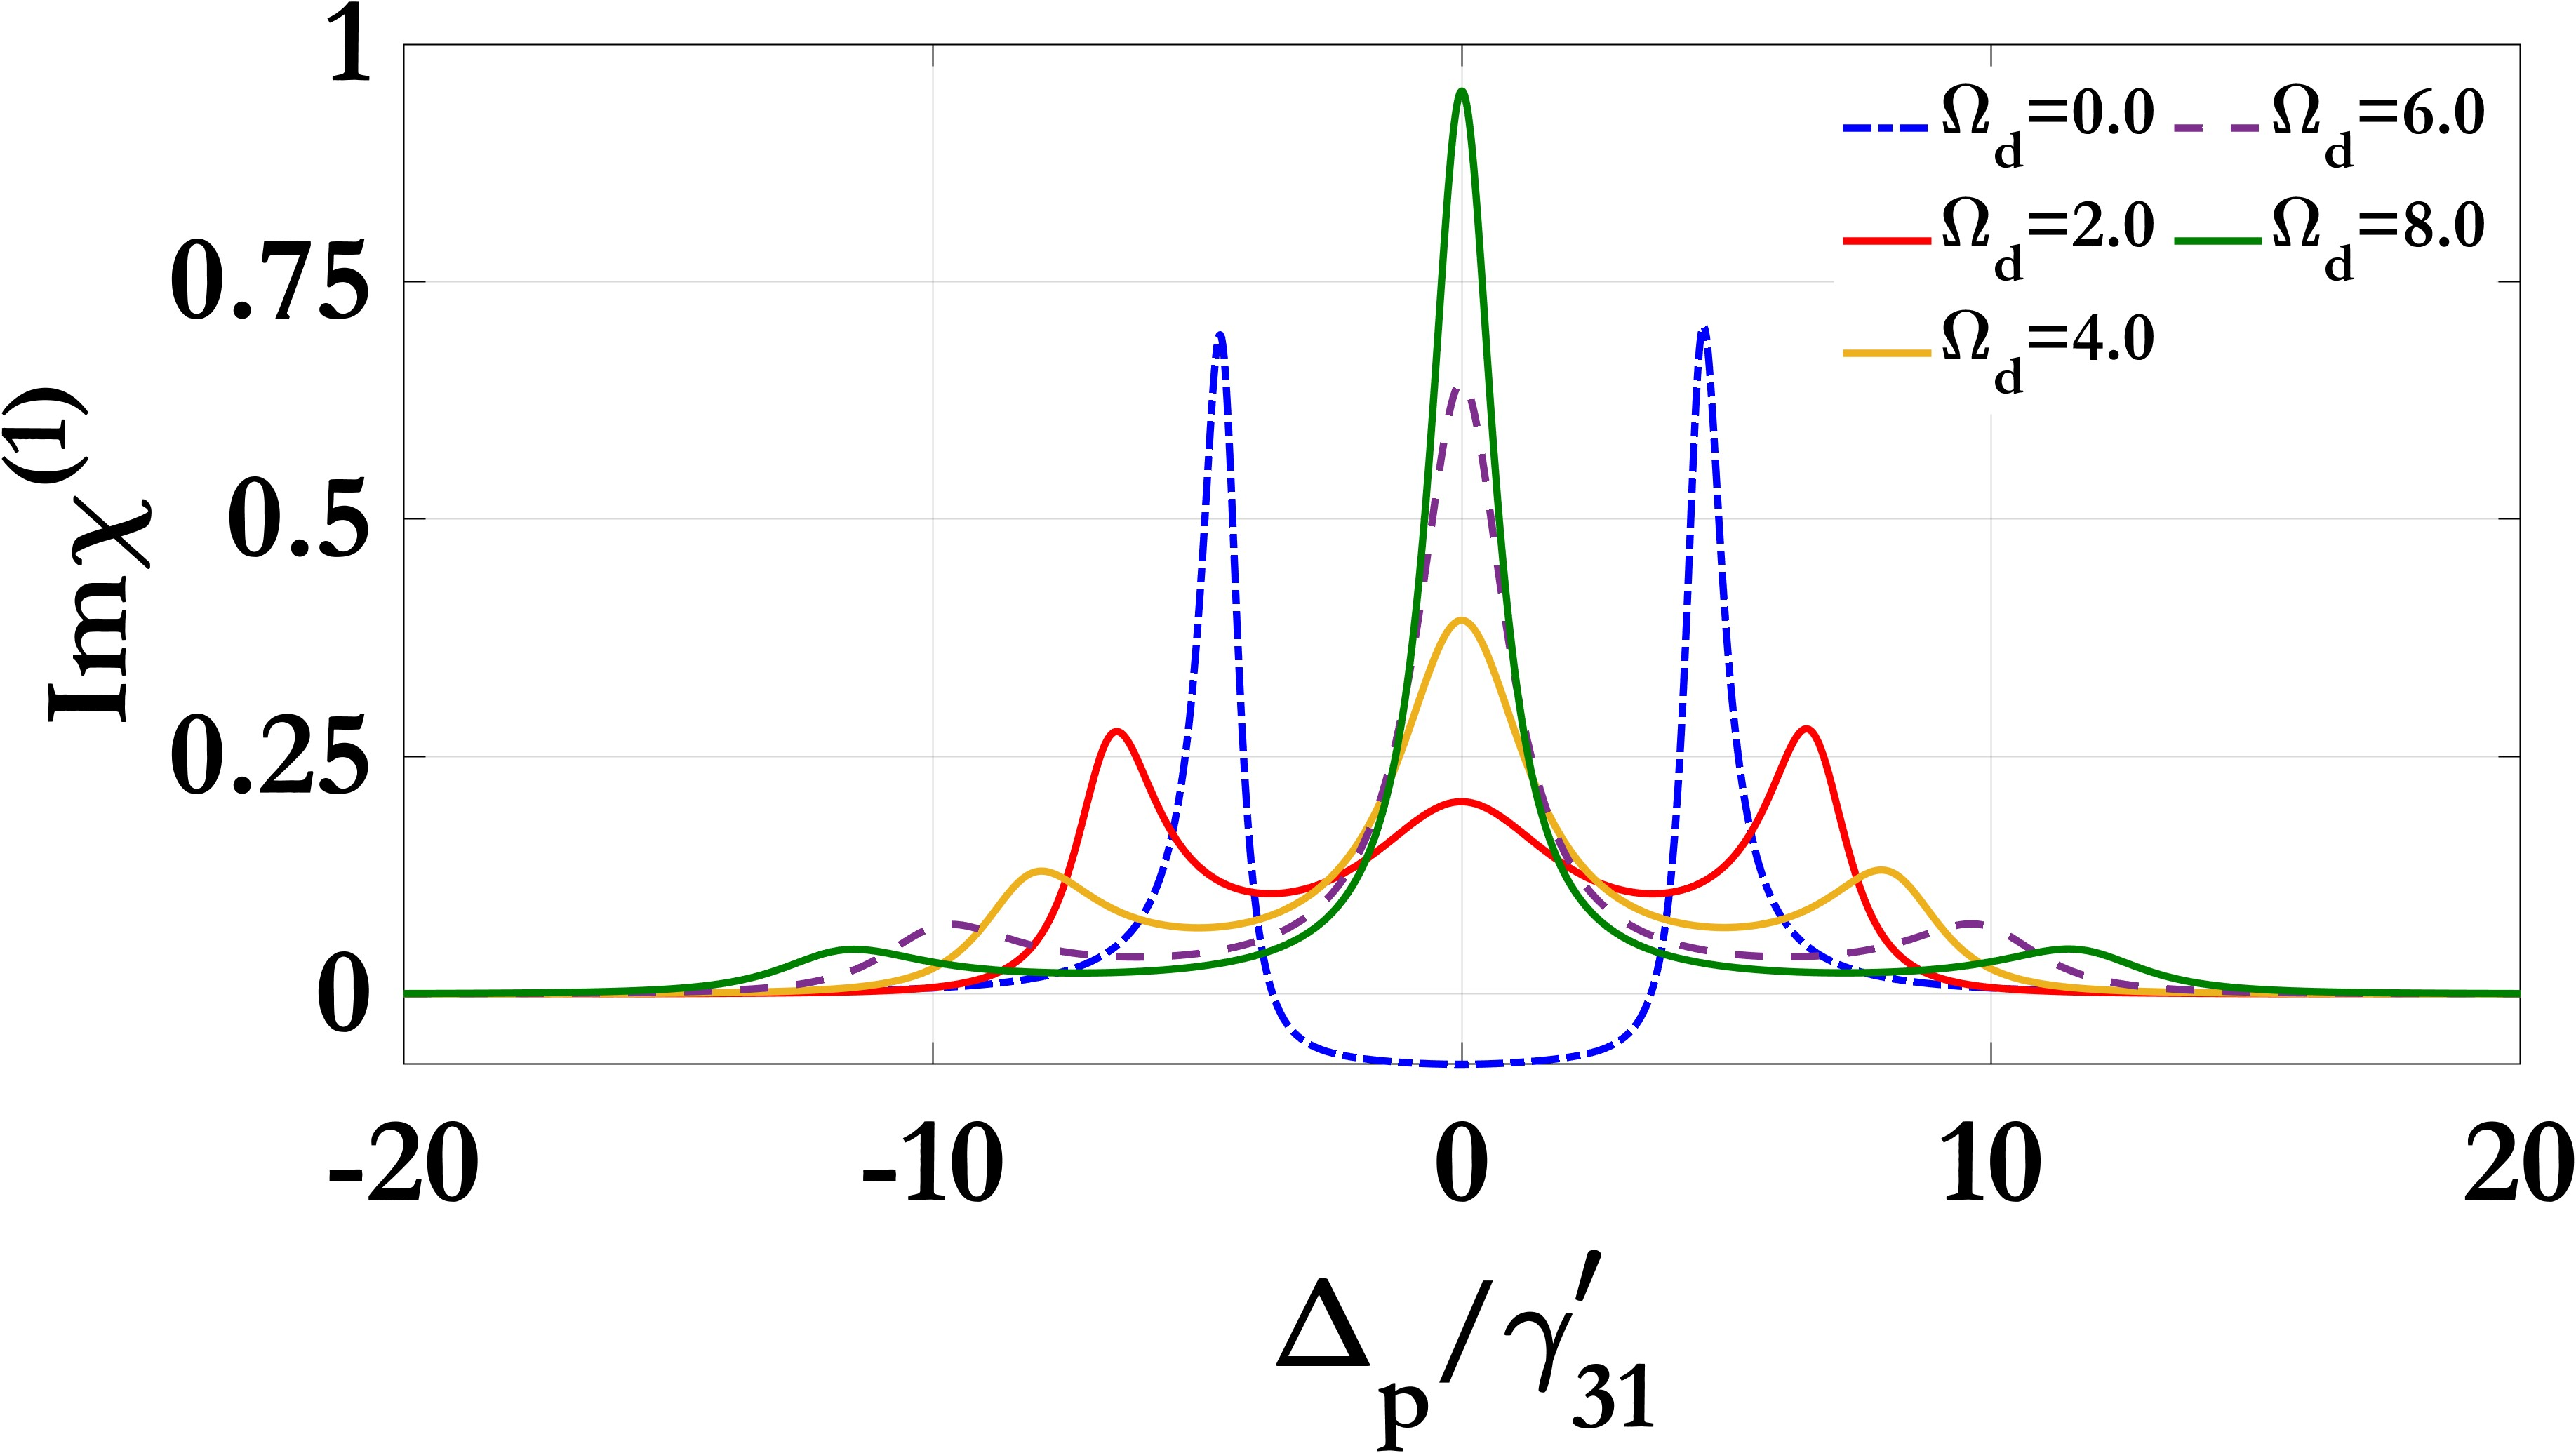
\includegraphics[width=\linewidth]{Plots/Img_chi1_Omega_d.jpeg}
    \subcaption{}
  \end{minipage}%
  \hfill
  \begin{minipage}[t]{0.48\textwidth}
    \centering
    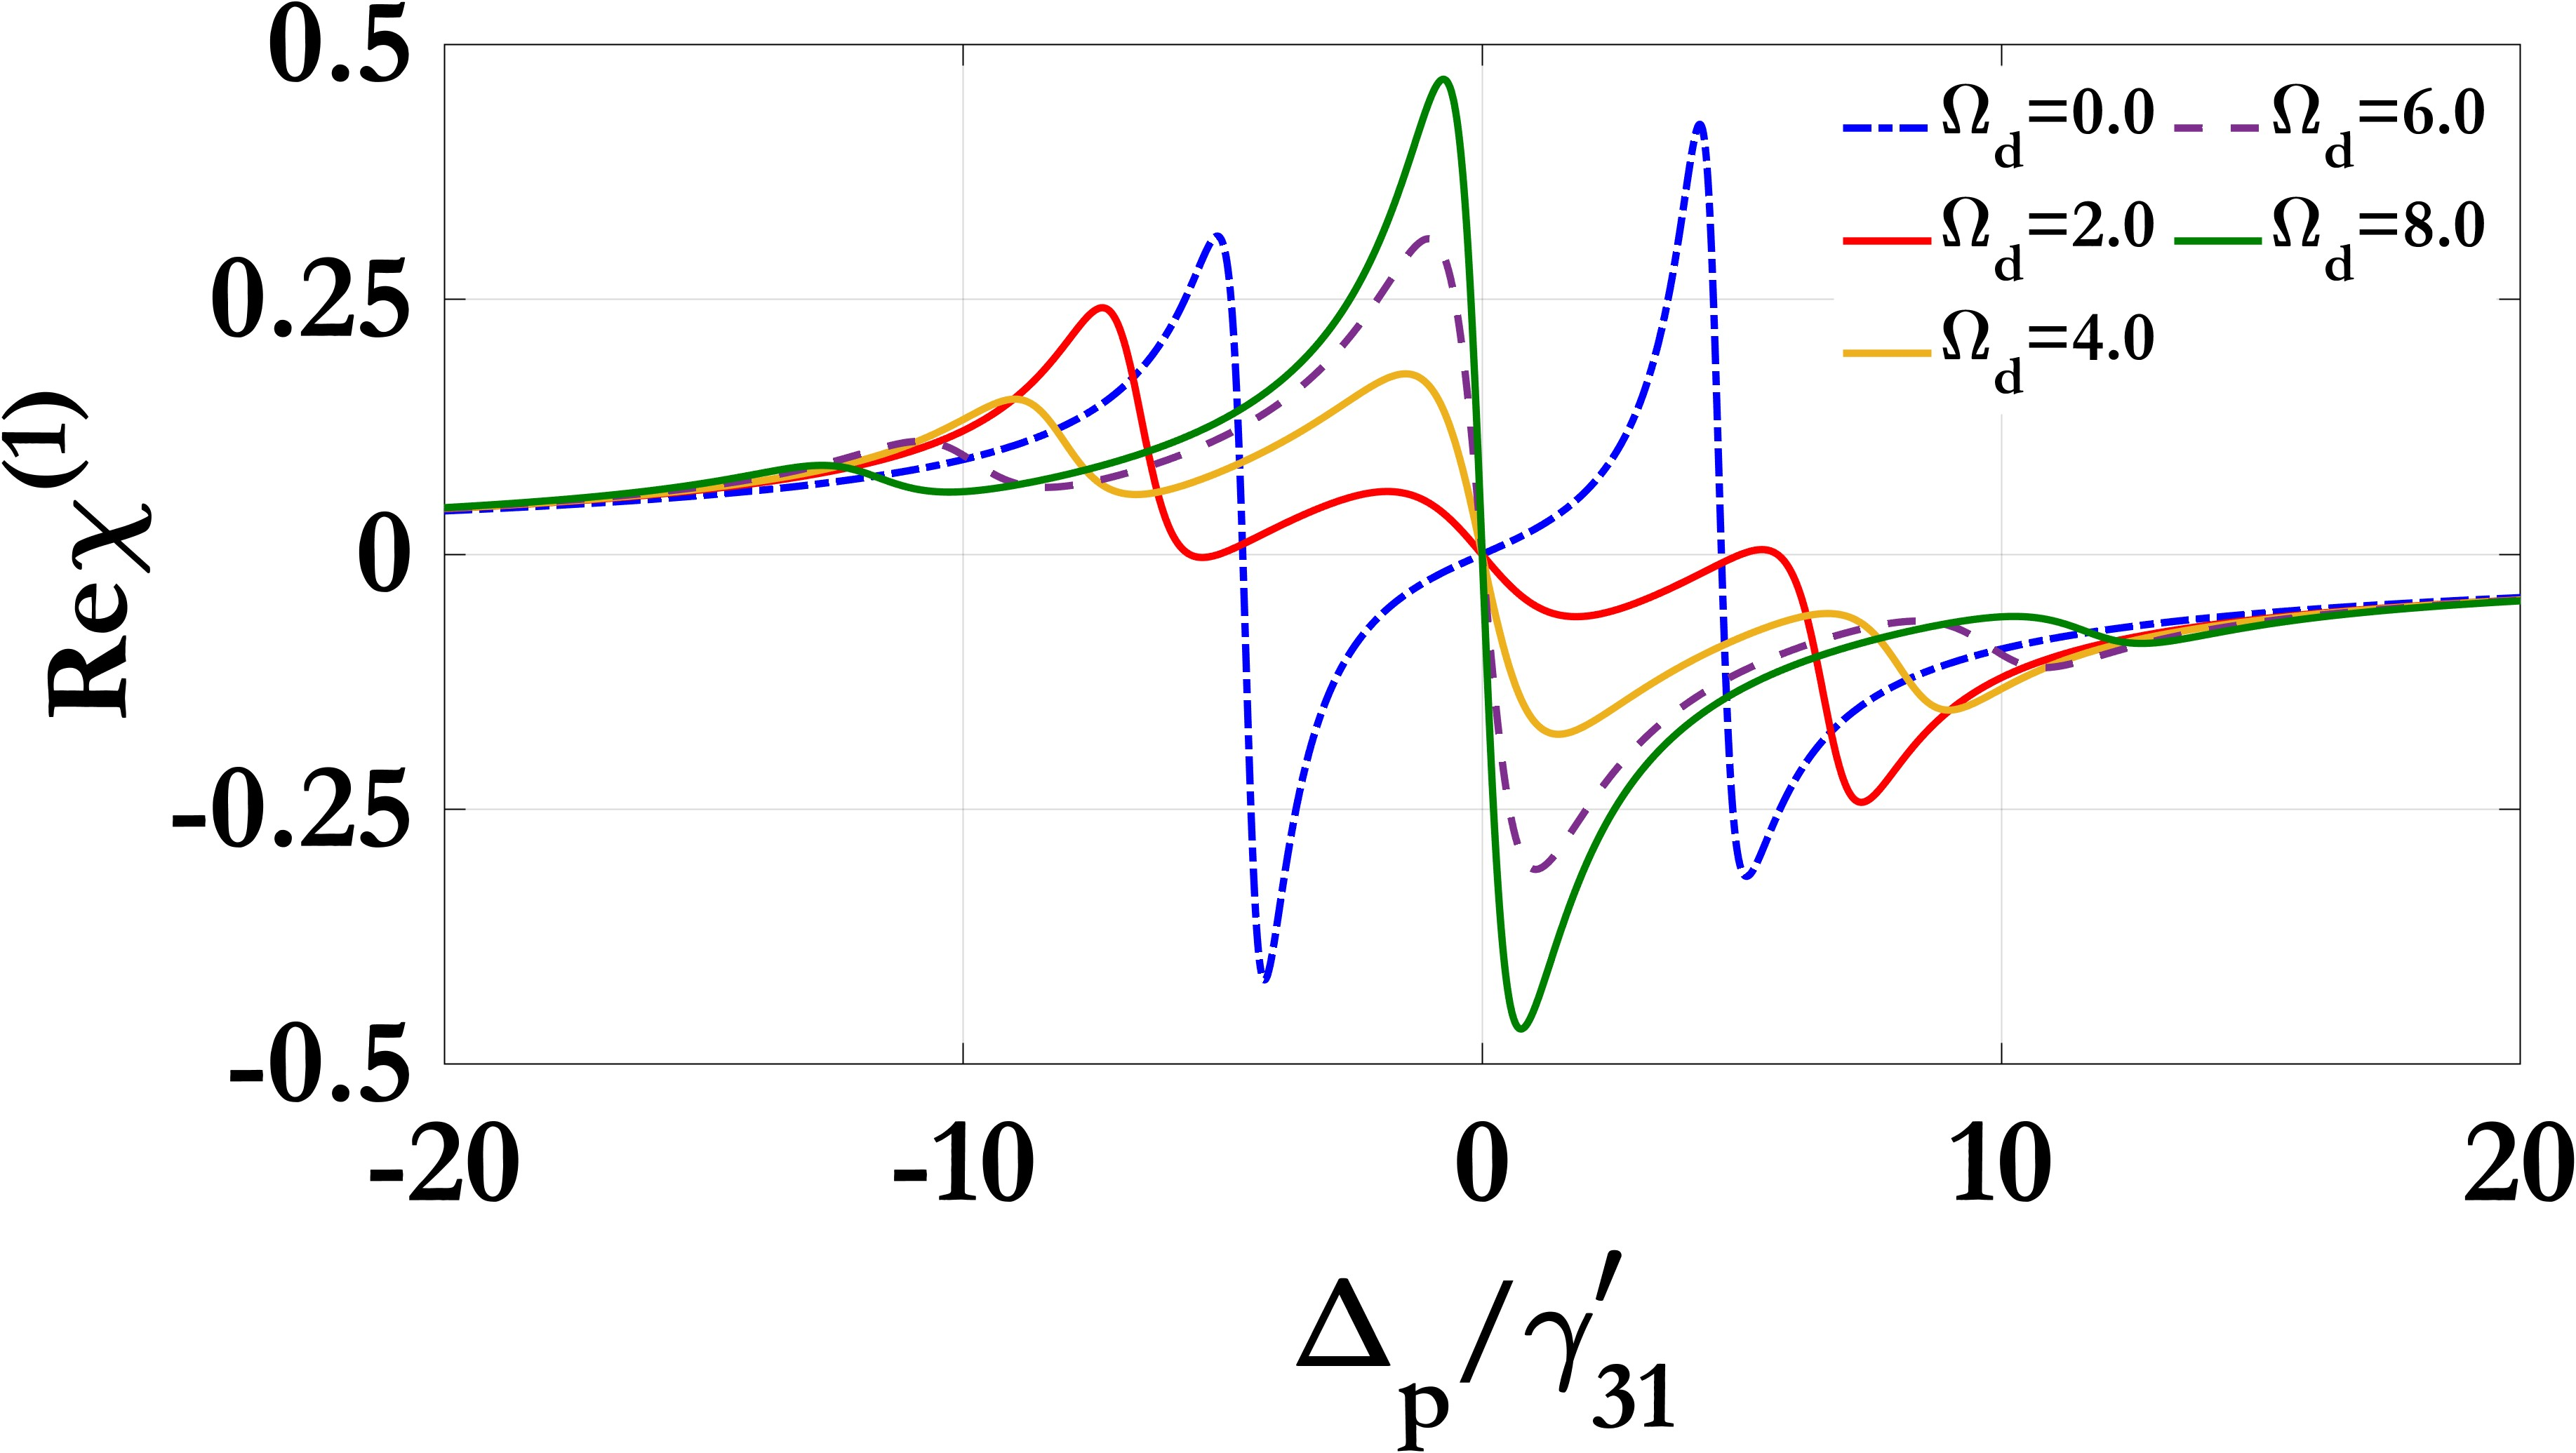
\includegraphics[width=\linewidth]{Plots/Real_chi1_Omega_d.jpeg}
    \subcaption{}
  \end{minipage}
  \caption{Variation of the imaginary (a) and real (b) parts of linear susceptibility as a function of normalized probe detuning for different values of Rabi frequency of second control field ($\Omega_c=0\gamma^{\prime}_{31},\ 1\gamma^{\prime}_{31}$) for imaginary part and ($\Omega_c=2\gamma^{\prime}_{31}$) for real part and Rabi frequency of the third control field is switched off.}
  \label{fig:omegad}
\end{figure}

In this section we examine the behaviour of linear, Kerr nonliniearities exhibited by multiple SQD-systems at the probe frequency. The value of the several parameters releated to the SQDs are as follows \(\mu_{41} = 15.68\times10^{-29} Cm\), \(\omega_p = 2.84\times10^{14} S^{-1}\). The decay rates are \(\gamma_{21}=3\times10^9S^{-1}\), \( \gamma_{31}=2\times10^9S^{-1} \), \( \gamma_{41}=4.1\times10^{11}S^{-1} \), and the value of the normalization constant is chosen to be \( \gamma^{\prime}_{31}=1\ ps^{-1} \). In Fig.1(a) we have depicted the variations of the imaginary part of the linear susceptibility with normalized probe detuning ($\Delta_p/\gamma^{\prime}_{31}$) for different values of Rabi frequency of first control field is kept constant at $\Omega_c/\gamma^{\prime}_{31}=0$ and $\Omega_d/\gamma^{\prime}_{31}=1$ and third control field ($\Omega_b$) is switched off. From Fig.1(a), under the resonance (i.e., $\Delta_c = \Delta_b = \Delta_d = 0$), it has shown that in the absence of second control field (i.e., $\Omega_d = 0$) the probe beam experiences large absorption at around $\Omega_p=0$. With the increase in the value of Rabi frequency of second control beam, the width of absorption peak gradually decrease, while side peaks emerges on both sides of the main peak. Consequently, transmission windows are created at the off-resonant positions ($\Delta_p \neq 0$) of the probe beam.The width of these two side windows increases with the increase of the value of $\Omega_d/\gamma^{\prime}_{31}$. Therefore the second control beam is not sufficient to create a transperency window at the probe resonance. Secondary transmission window can be created at off-resonant positions. Fig.1(b) demostrates the variation of the real part of $\chi^{(1)}$ versus normalized probe detuning ($\Delta_p/\gamma^{\prime}_{31}$) for different values of Rabi frequency ($\Omega_{d}$) of second control beam. While Rabi frequency of first and third control field is kept constant at $\Omega_{c}/\gamma^{\prime}_{31}=2$ and $\Omega_{b}/\gamma^{\prime}_{31}=2$.As shown in Fig.1(b) with the increase in the value of the second control beam $\Omega_{d}$ from $0$ to $8\gamma^{\prime}_{31}$, the slope of the ($Re\chi^{(1)}$) changes and since this slope determines the group velocity of the beam, consequently the group velocity can be controlled by second control beam. \par

\begin{figure}[ht]
  \centering
  \begin{minipage}{0.48\textwidth}
    \centering
    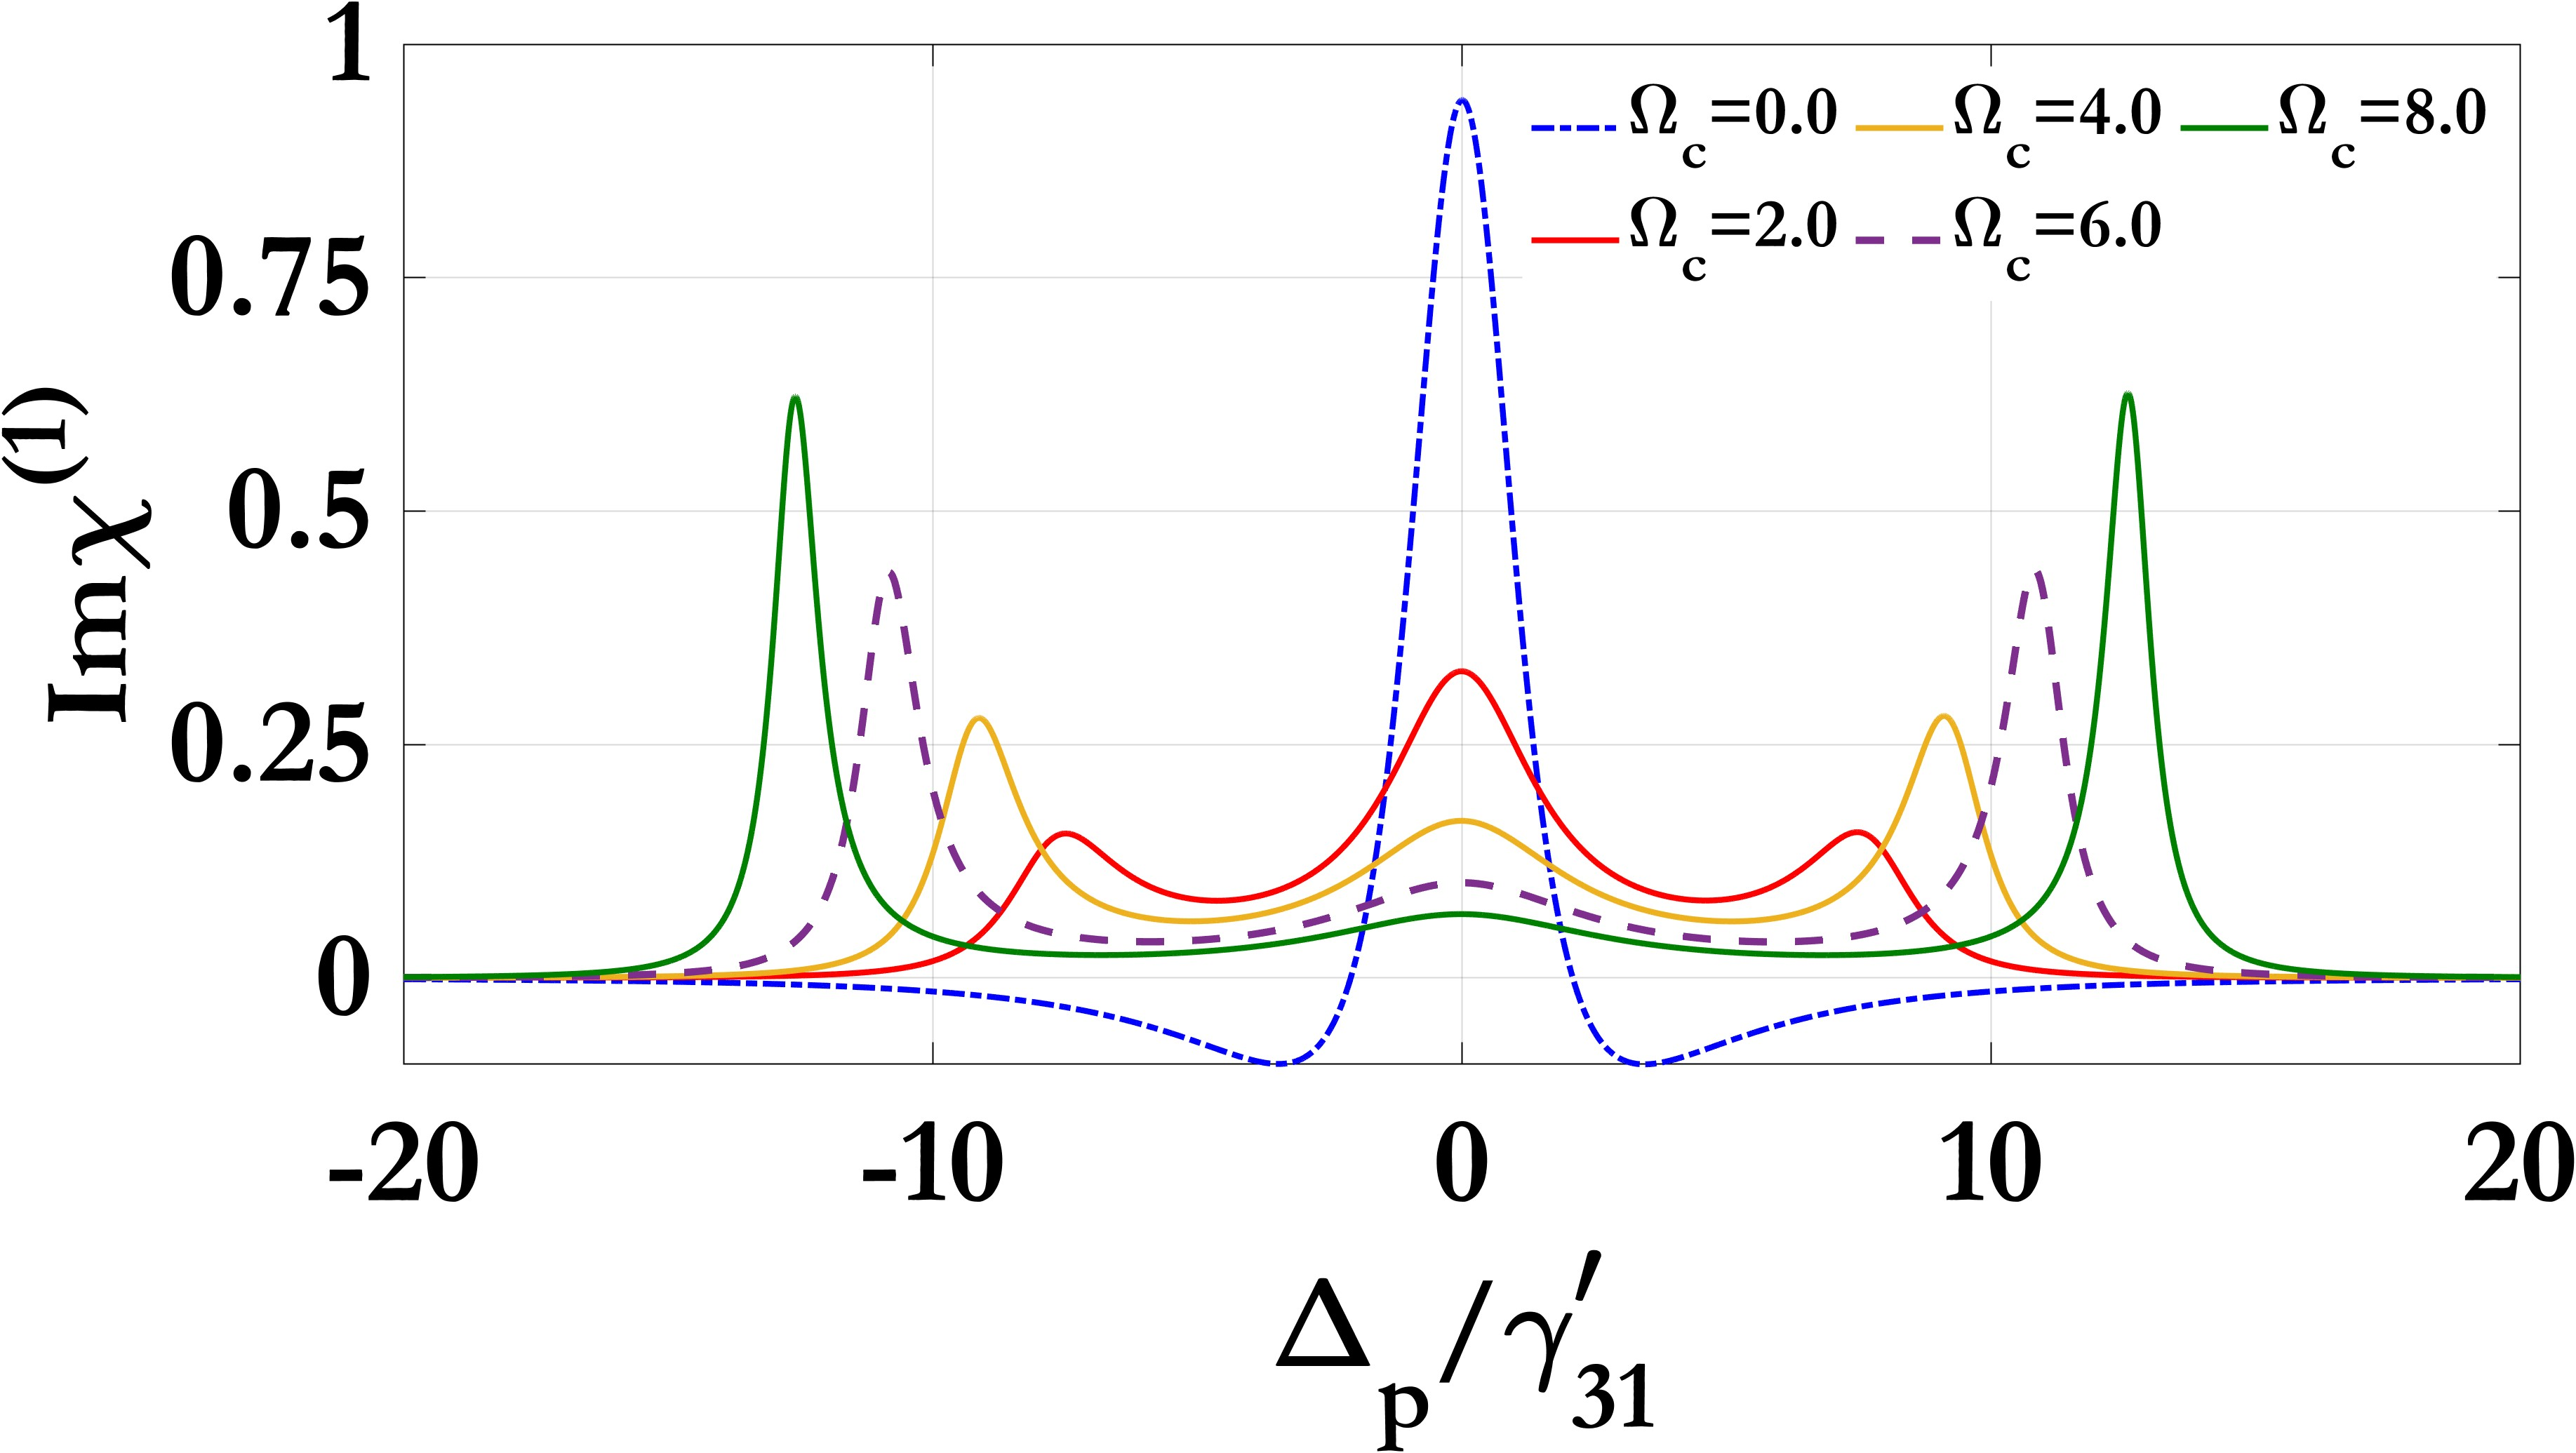
\includegraphics[width=\linewidth]{Plots/Img_chi1_Omega_c.jpeg}
    \subcaption{}
  \end{minipage}%
  \hfill
  \begin{minipage}{0.48\textwidth}
    \centering
    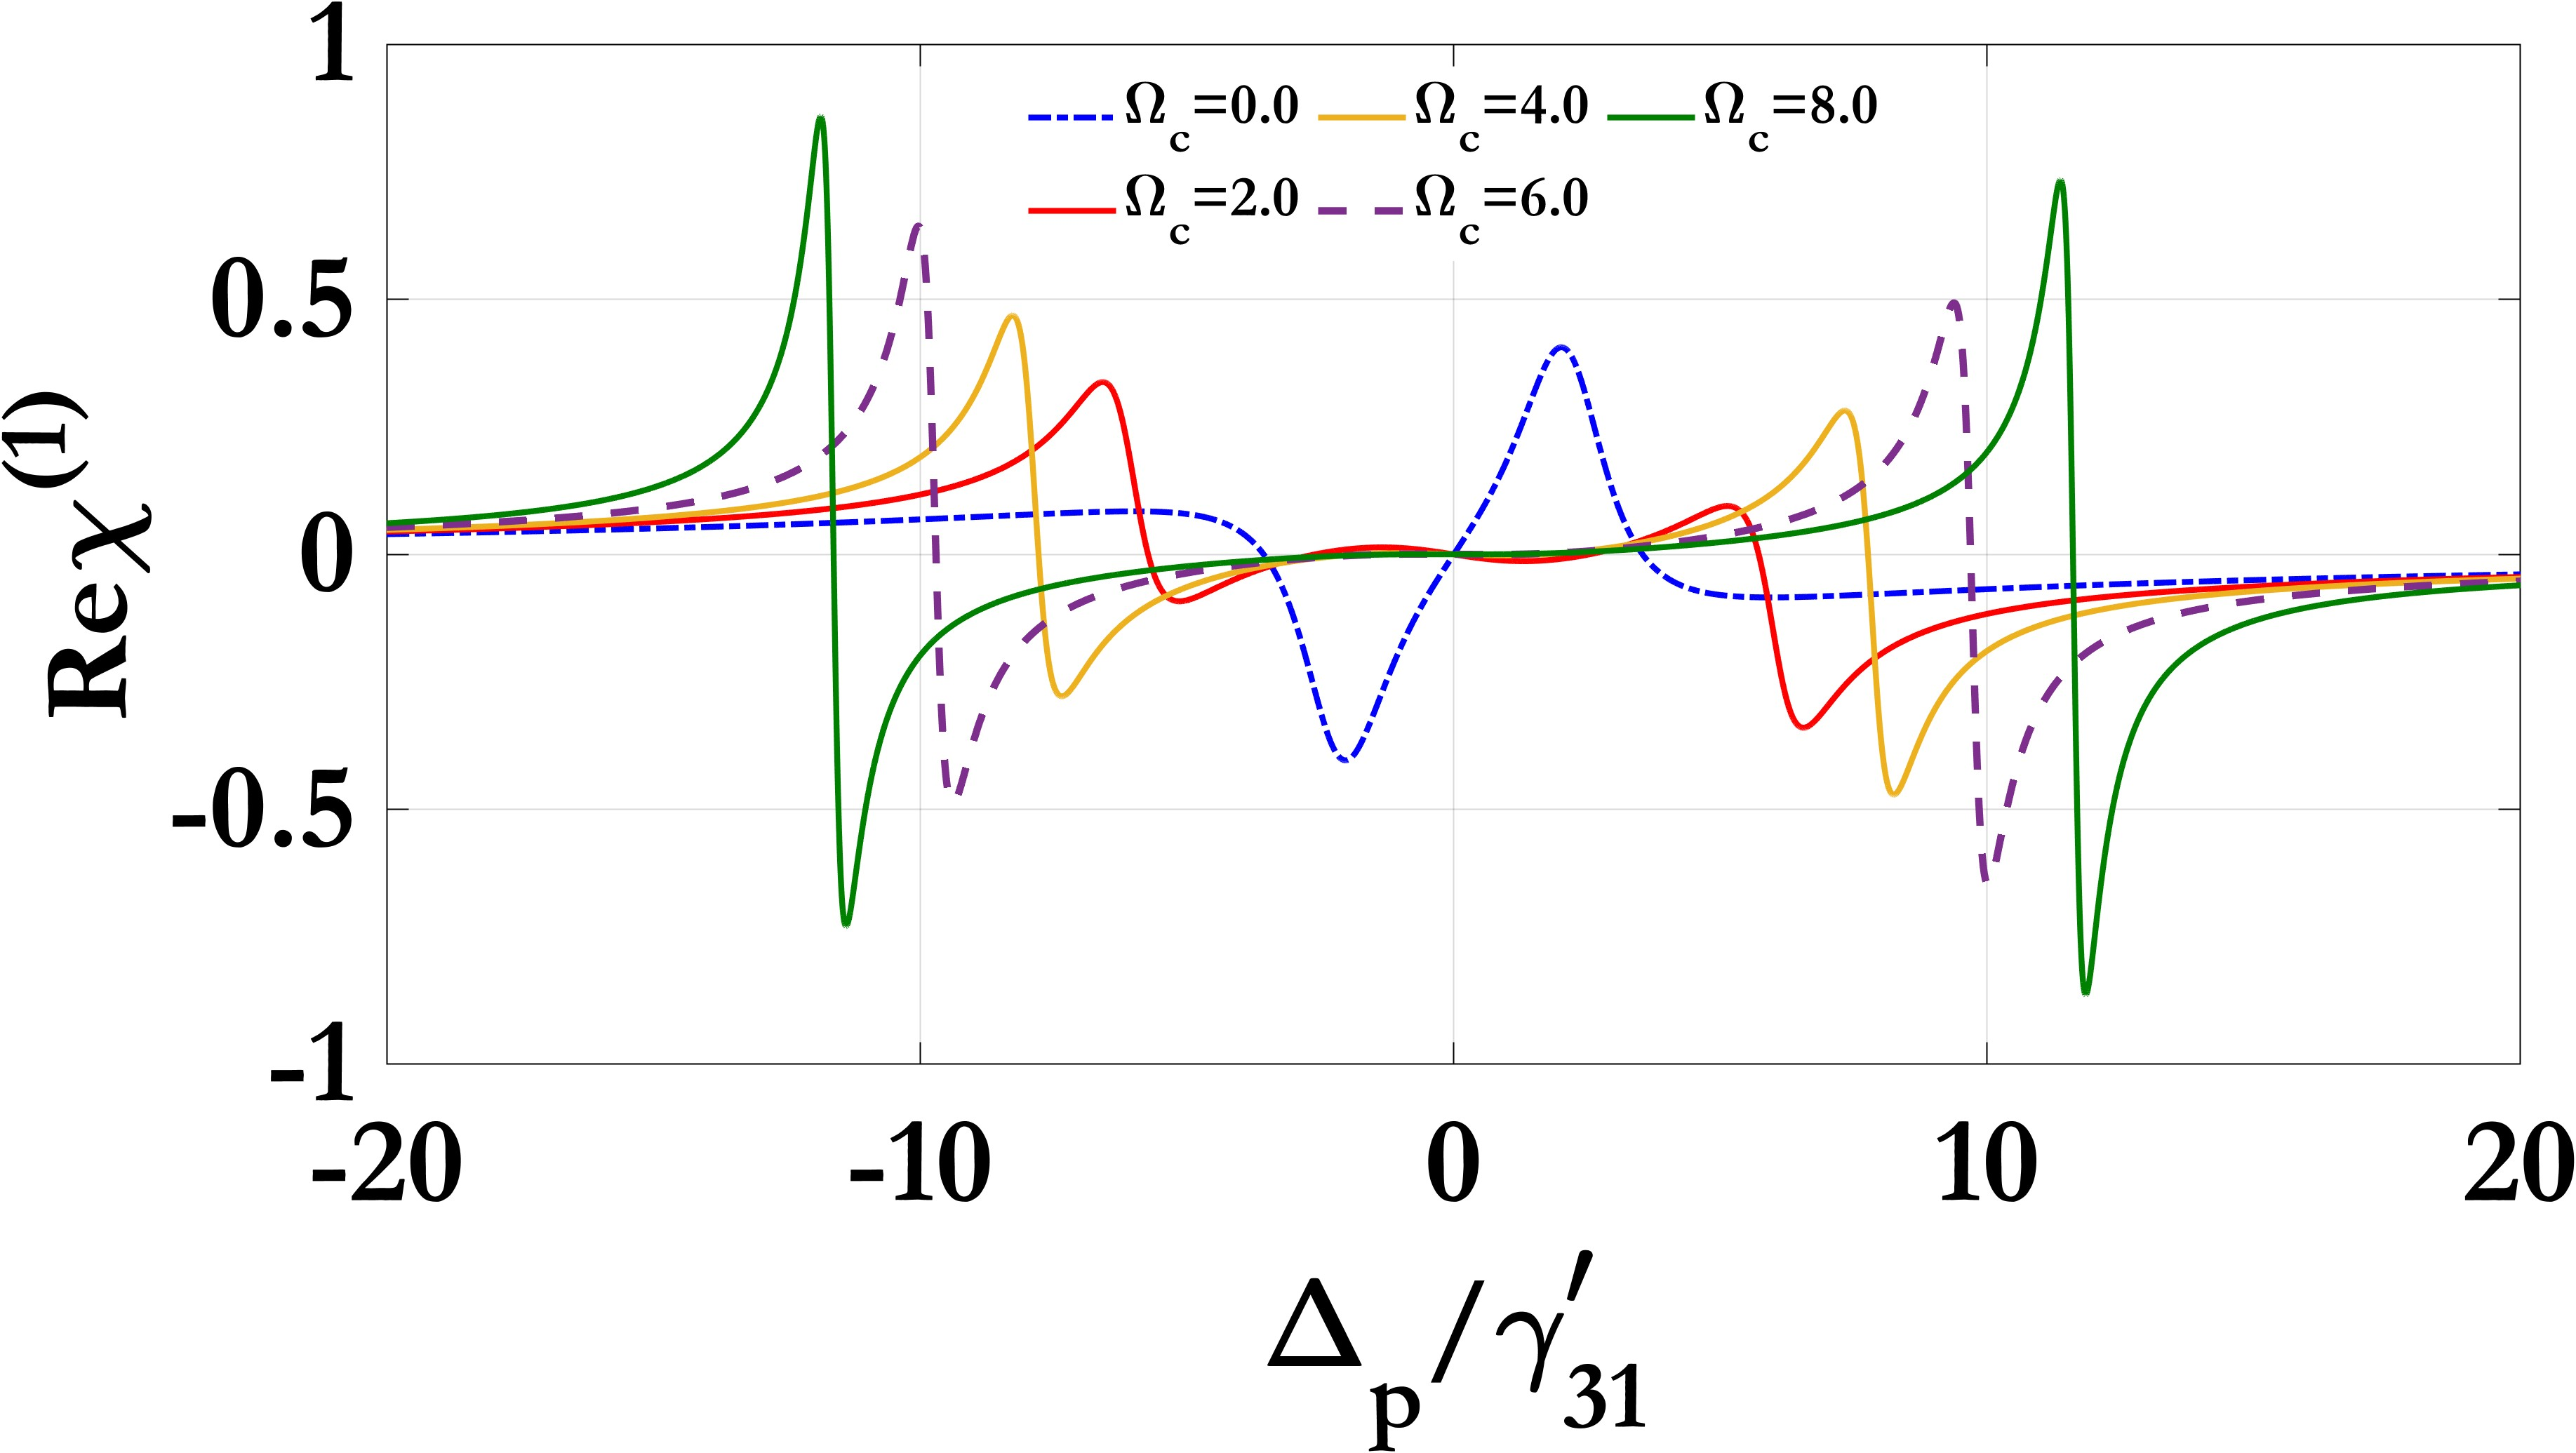
\includegraphics[width=\linewidth]{Plots/Real_chi1_Omega_c.jpeg}
    \subcaption{}
  \end{minipage}
  \caption{Variation of the imaginary (a) and real (b) parts of linear susceptibility as a function of normalized probe detuning for different values of Rabi frequency of second control field ($\Omega_c=0\gamma^{\prime}_{31},\ 1\gamma^{\prime}_{31}$) for imaginary part and ($\Omega_c=2\gamma^{\prime}_{31}$) for real part and Rabi frequency of the third control field is switched off.}
  \label{fig:real_omegac}
\end{figure}

We now examine the influence of first control field ($\Omega_{c}$) on the behaviour of linear susceptibility. We have discussed the variations of the imaginary and real part of $\chi^{(1)}$ with normalized probe $\Delta_{p}/\gamma^{\prime}_{31}$ for different values of the Rabi frequency of the first control beam ($\Omega_c$), while the values of other two control field kept constant (i.e. switched off).

From Fig.2(a) we notice that absorption window is created at $\Omega_{c}=0$ when second and third control field are switched off (i.e. $\Omega_{d}=\Omega_{b}=0$). As a result of increasing the value of $\Omega_{c}$ the height of the absorption window is gradually decreasing and also a secondary transparency window is created and the width of the transparency window is increased for higher value of $\Omega_{c}$ and also the height of the transparency window decreases. On the other hand, from Fig. 2(b) we find that slope of real $\chi^{(1)}$ changes from negative in the domain $-0.5 \leq \Delta_{p}/\gamma^{\prime}_{31} \leq 0.5$ for $\Omega_{C}/\gamma^{\prime}_{31}=0$ and similar behaviour is observed for the other cases of $\Omega_{c}$.

The influence of the first control field Rabi frequency $\Omega_c$ on the linear susceptibility $\chi^{(1)}$ reveals significant insights into the coherent dynamics of the atomic system. As shown in the real part of the susceptibility, $\mathrm{Re}[\chi^{(1)}]$, an increase in $\Omega_c$ leads to a clear dispersive splitting near the probe detuning $\Delta_p = 0$. At low $\Omega_c$, the dispersion remains broad and relatively featureless, but as $\Omega_c$ is increased, sharp dispersion profiles emerge, with zero crossings shifting symmetrically outward from the origin. This behavior reflects the dressing of atomic levels due to the strong coupling field, where the energy eigenstates of the system split, and their interference leads to pronounced refractive index modulation. Such steep dispersion features are particularly relevant for applications in slow light and enhanced nonlinear optics, where the group velocity and susceptibility gradient play a pivotal role.

In parallel, the imaginary part $\mathrm{Im}[\chi^{(1)}]$, which governs absorption, displays a transition from a single absorption peak at low $\Omega_c$ to a pronounced transparency window as $\Omega_c$ increases. This transparency---centered at $\Delta_p = 0$---emerges from destructive quantum interference between excitation pathways, a hallmark of Electromagnetically Induced Transparency (EIT). As $\Omega_c$ becomes large, the absorption profile evolves into a doublet structure with peaks at detunings proportional to $\Omega_c$. This play of EIT, modulated by the control field strength, offers a tunable platform for manipulating light--matter interactions, thereby enabling dynamic control over absorption and dispersion in multi-level atomic media.

\begin{figure}[h]
  \centering
  \begin{minipage}{0.48\textwidth}
    \centering
    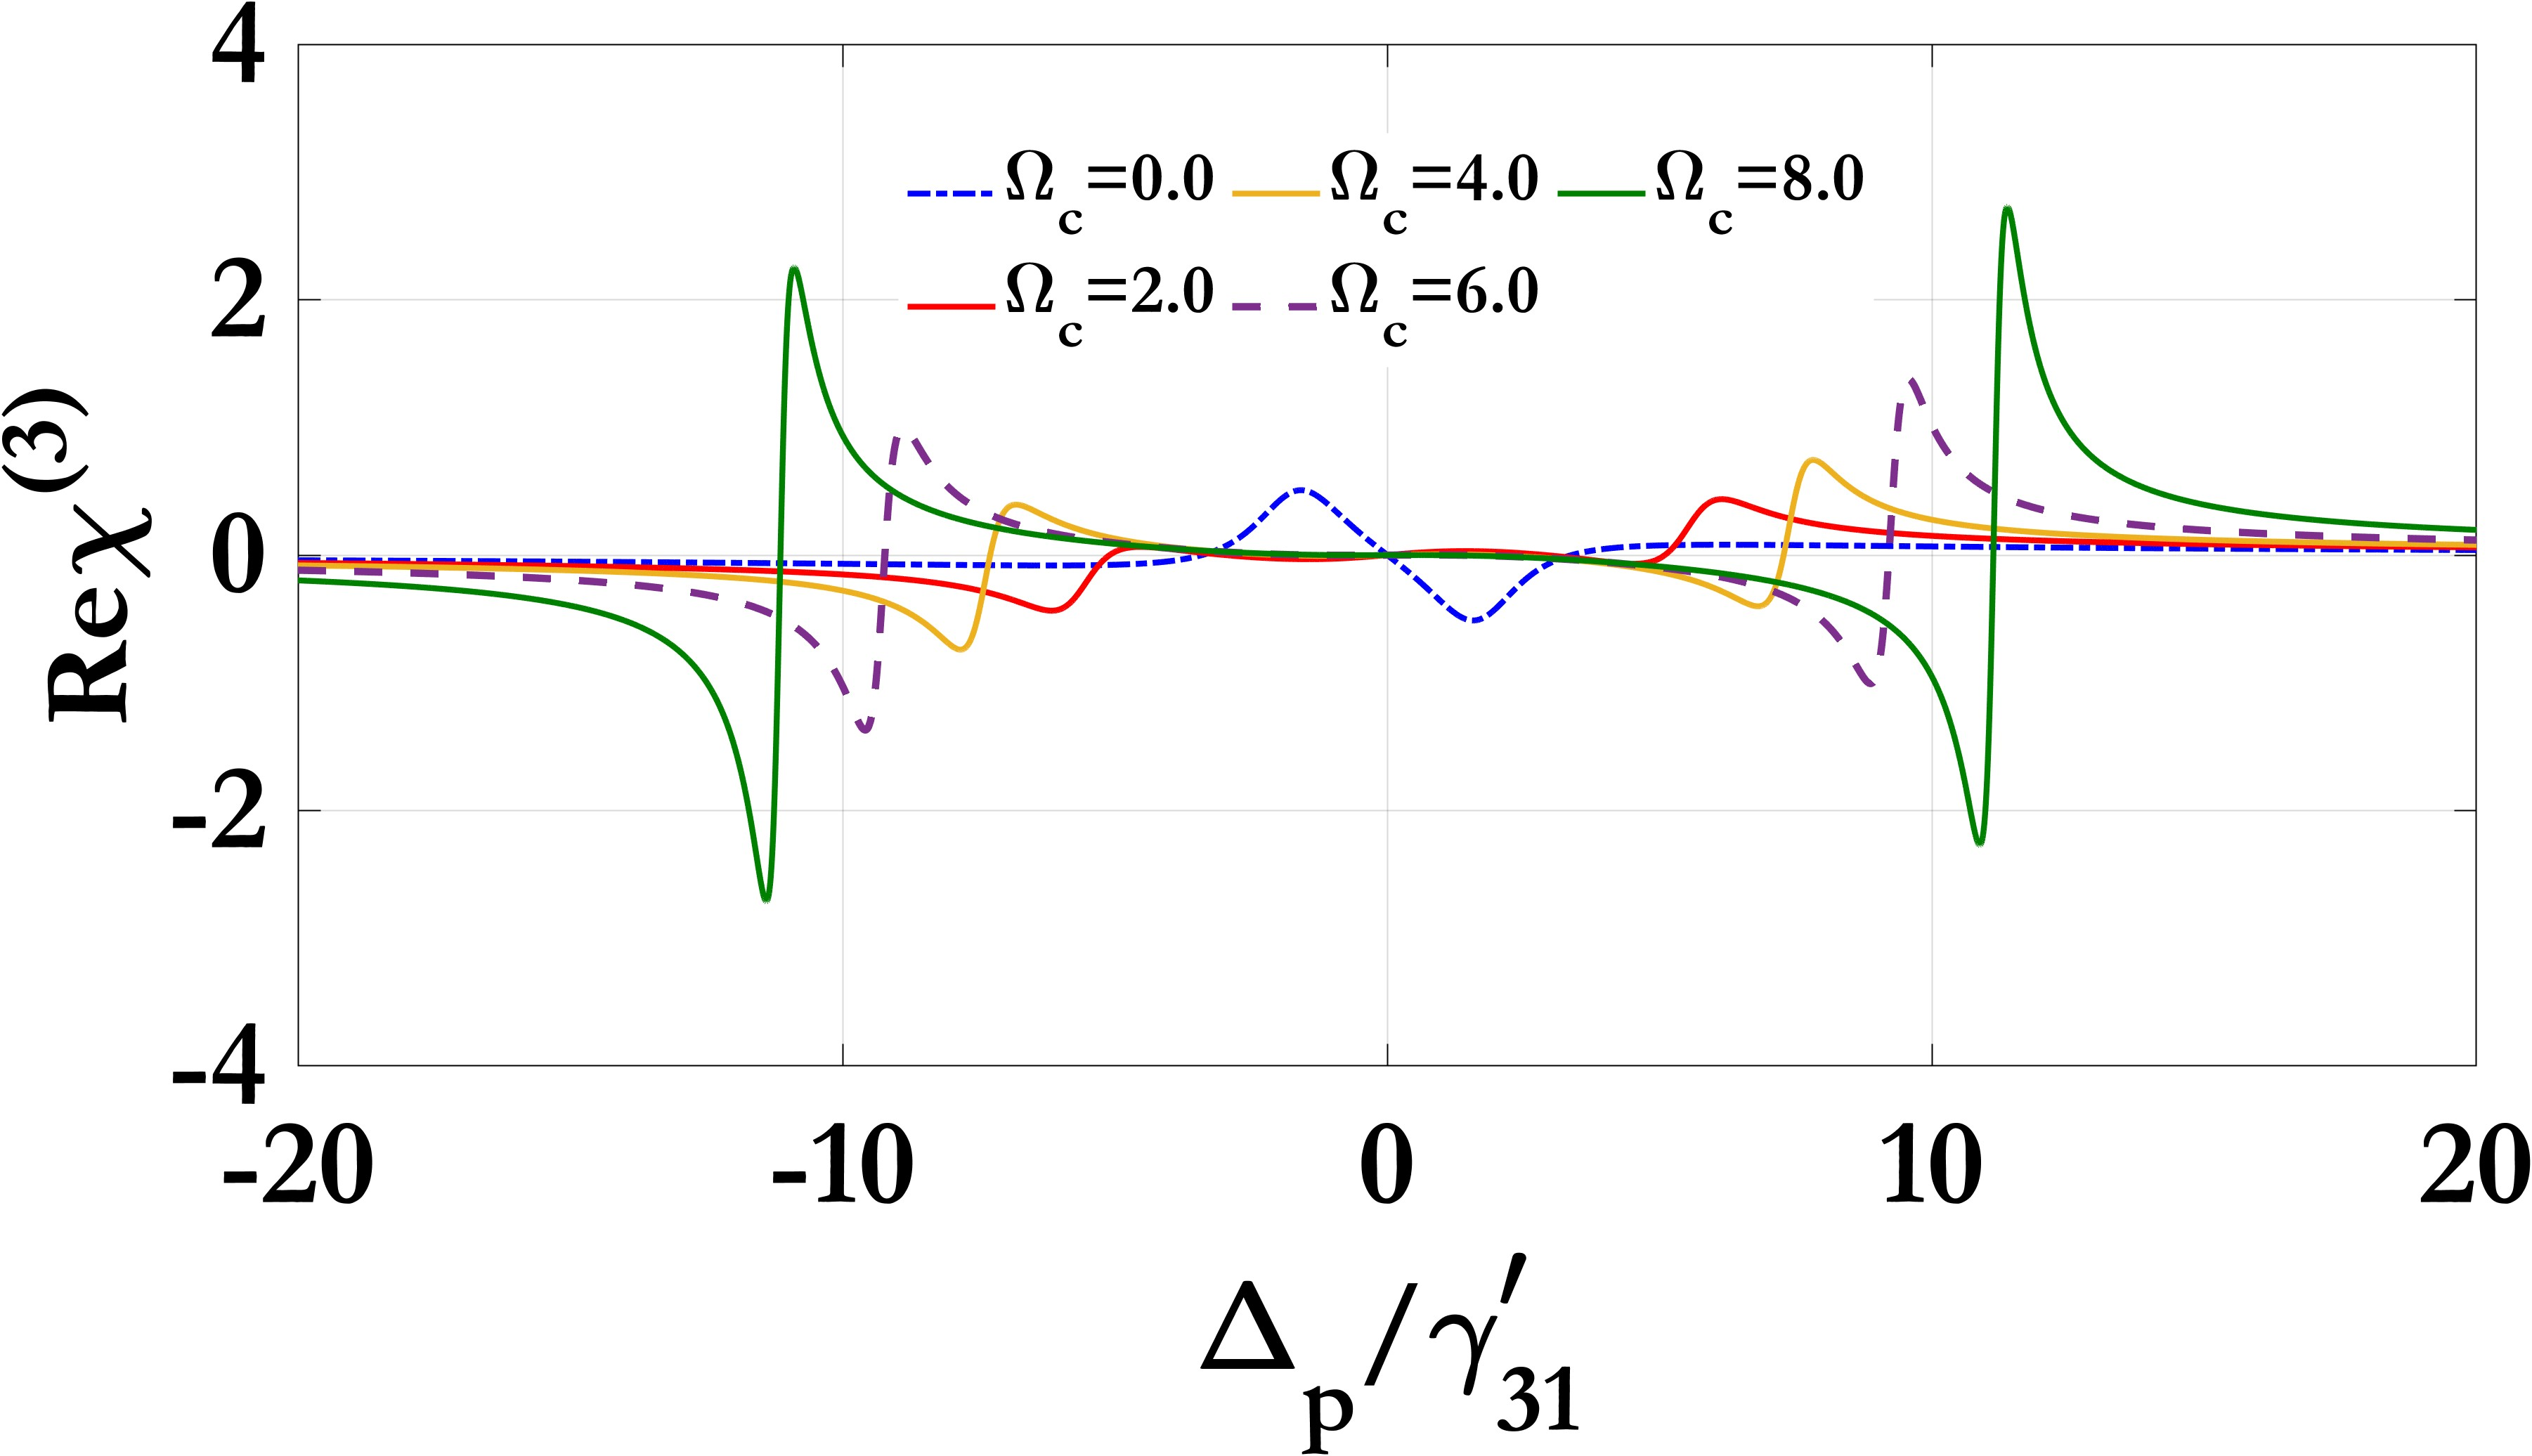
\includegraphics[width=\linewidth]{Plots/Real_chi3_Omega_c.jpeg}
    \subcaption{}
  \end{minipage}%
  \hfill
  \begin{minipage}{0.48\textwidth}
    \centering
    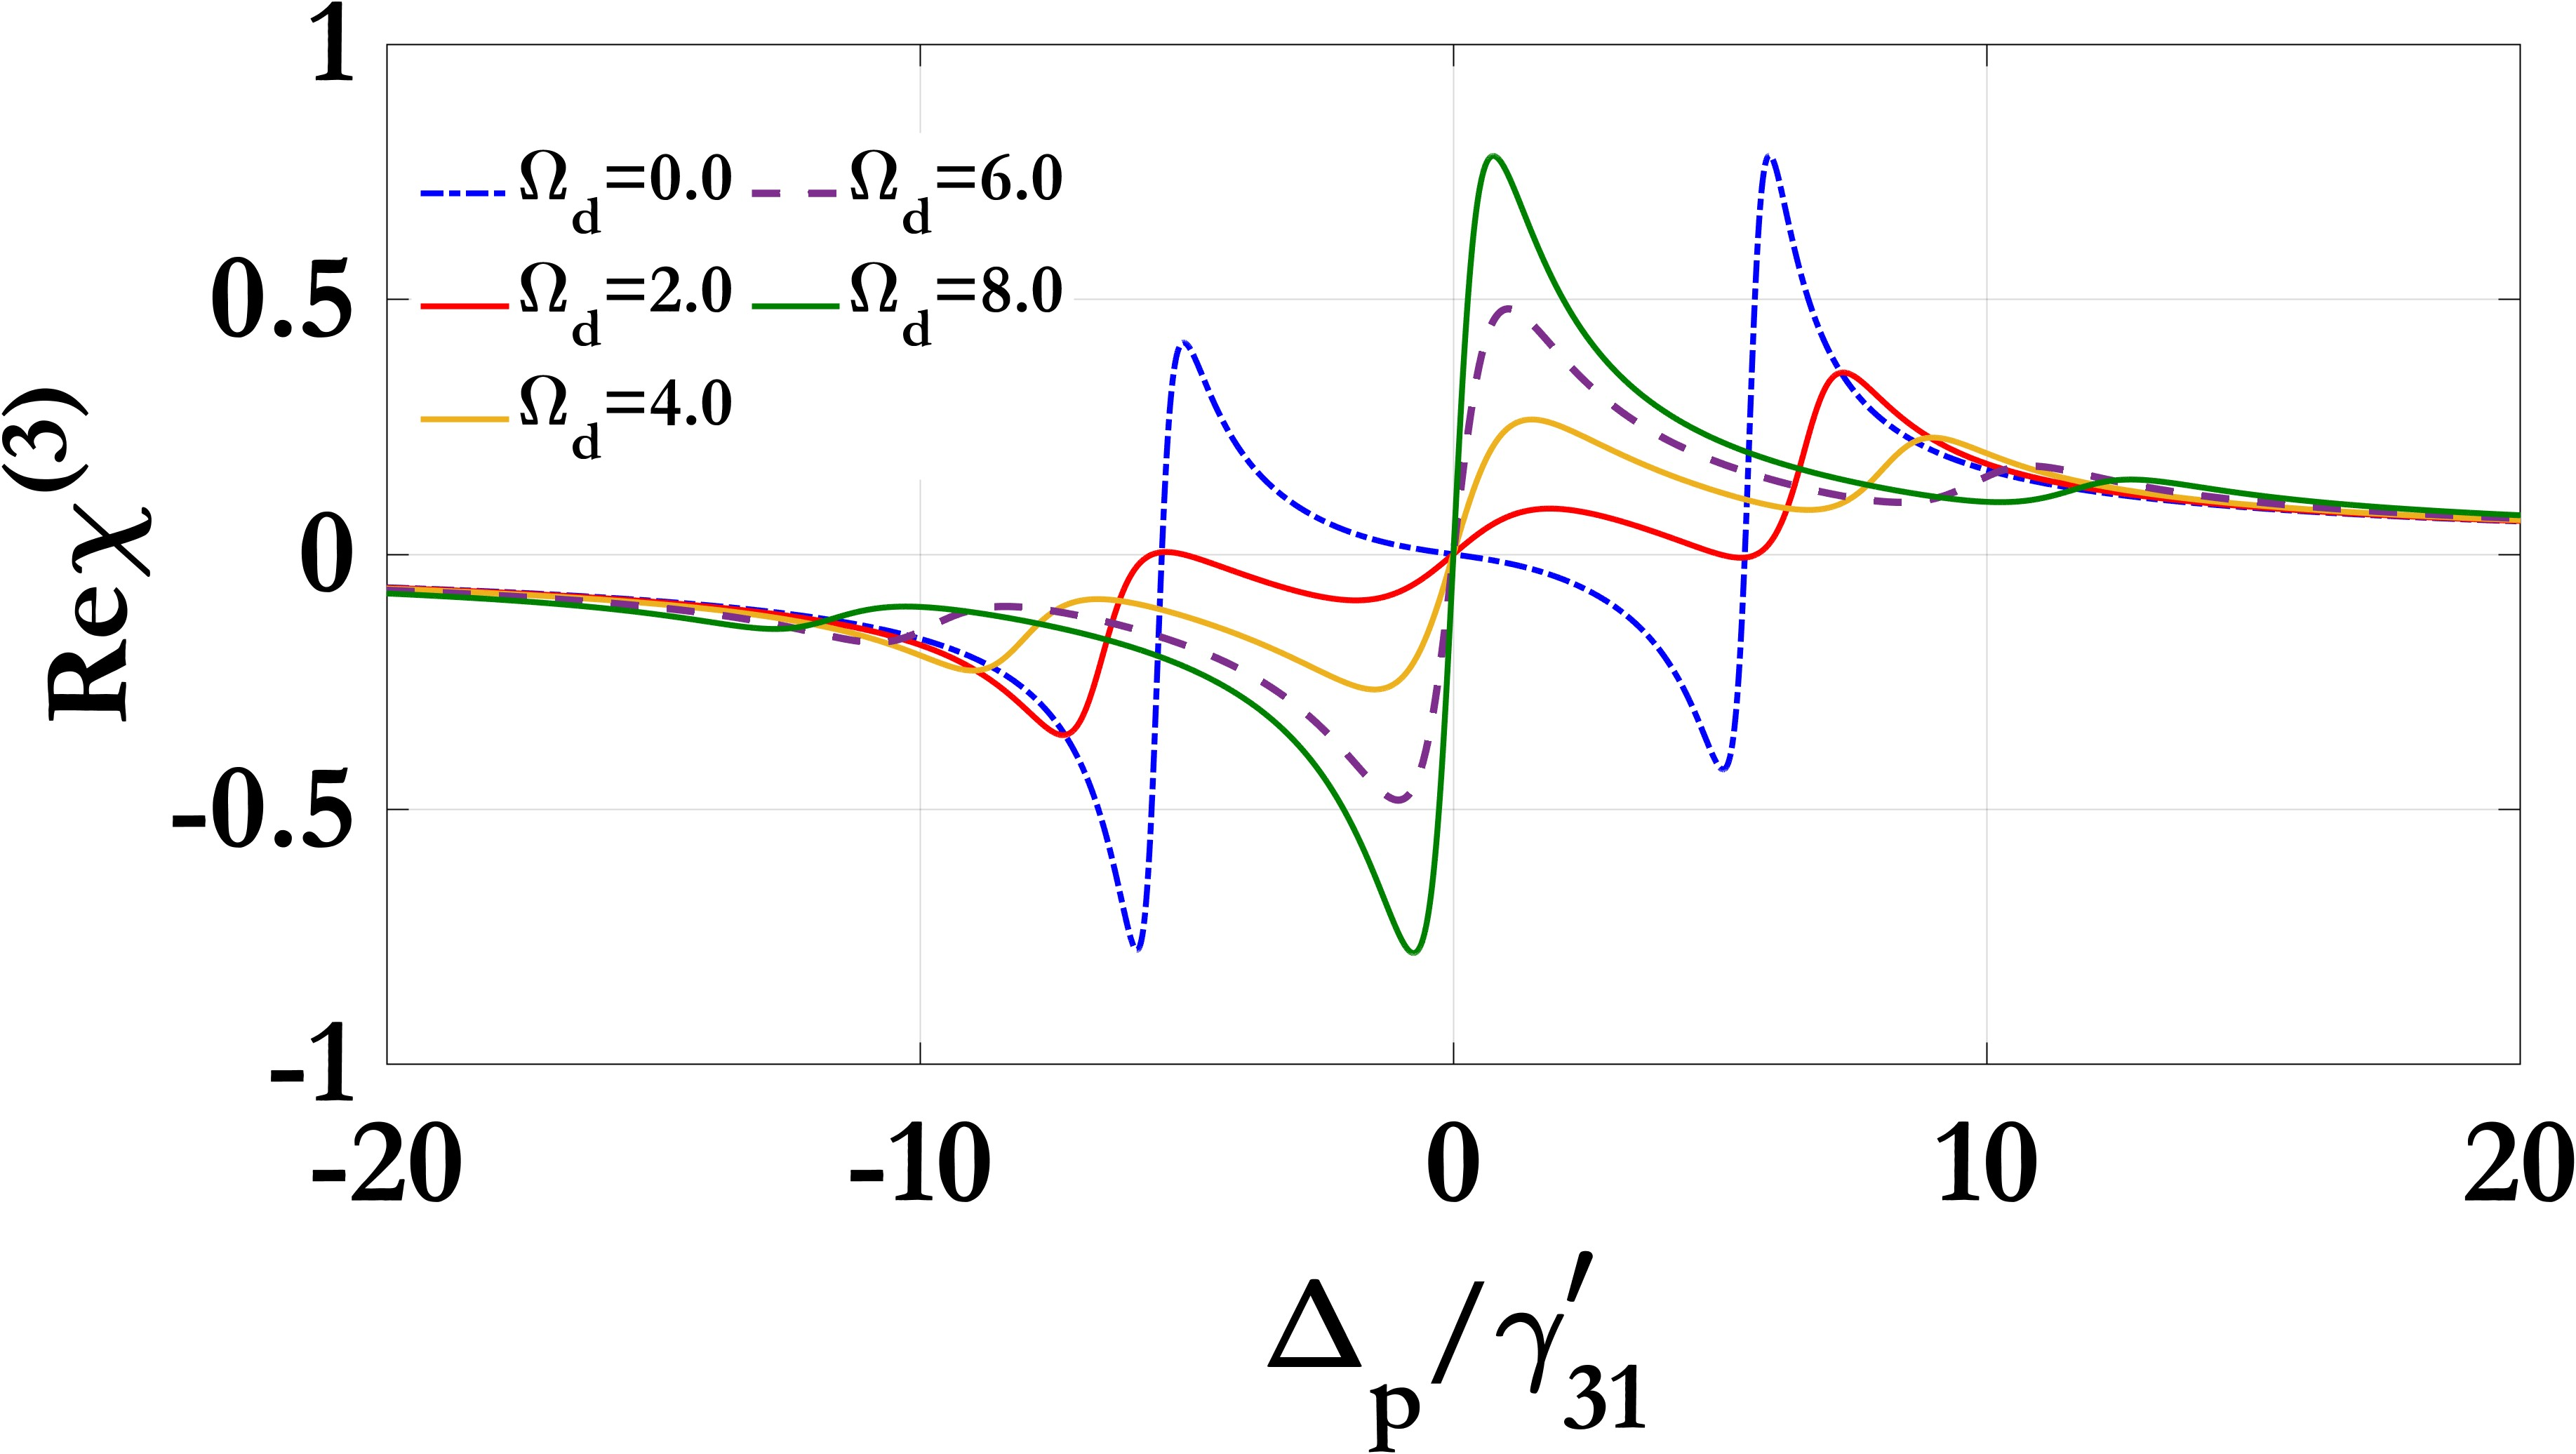
\includegraphics[width=\linewidth]{Plots/Real_chi3_Omega_d.jpeg}
    \subcaption{}
  \end{minipage}
  \caption{Variation of the imaginary (a) and real (b) parts of linear susceptibility as a function of normalized probe detuning for different values of Rabi frequency of second control field ($\Omega_c=0\gamma^{\prime}_{31},\ 1\gamma^{\prime}_{31}$) for imaginary part and ($\Omega_c=2\gamma^{\prime}_{31}$) for real part and Rabi frequency of the third control field is switched off.}
  \label{fig:omegac}
\end{figure}

The dispersion spectra of the real part of the third-order nonlinear susceptibility, \(\text{Re}\,\chi^{(3)}\), presented in Figs.~X(a) and X(b), provide crucial insight into the underlying nonlinear optical response of the medium under varying Rabi frequencies of the dressing field \(\Omega_d\) and control field \(\Omega_c\), respectively. The system is considered under the fixed detuning conditions \(\Delta_c = 1\), \(\Delta_b = 2\), and \(\Delta_d = 0\), with the normalization factor \(\gamma_{41}^\prime = 1~\text{ps}^{-1}\). These dispersion profiles reveal significant sensitivity of the real part of \(\chi^{(3)}\) to the external driving fields, reflecting the tunable nature of the Kerr-type nonlinearity via coherent field control. As \(\Omega_d\) and \(\Omega_c\) are varied, one observes pronounced dispersive features—including polarity flips and sharp peaks—indicative of enhanced multi-photon coherence and interference effects among dressed atomic states. These features correspond to rapid variations in the refractive index and group velocity dispersion, which are foundational for phase-sensitive nonlinear phenomena such as four-wave mixing and cross-phase modulation.

More specifically, increasing \(\Omega_d\) or \(\Omega_c\) results in enhanced splitting and asymmetry in the dispersion profiles, a manifestation of strong Autler--Townes splitting and dynamic Stark shifts in the atomic energy levels. The observed spectral modulations point to the presence of both normal and anomalous dispersion regions, corresponding respectively to subluminal and superluminal group velocity regimes. Importantly, the field-dependent tailoring of \(\text{Re}\,\chi^{(3)}\) opens avenues for precise engineering of nonlinear optical responses, crucial for developing applications such as all-optical switching, tunable delay lines, and quantum phase gates. The ability to dynamically control the third-order susceptibility without introducing significant absorption further emphasizes the practicality of this scheme in low-power, high-coherence quantum photonic systems.

\section{Non-linear Schr\"{o}dinger Equation}
In order to study the modulation instability of the probe beam,which could be either a continuous wave (CW) or a quasi continuous wave(QCW), we need to derive an appropriate nonlinear Schrodinger equation~\cite{Scully_Zubairy_1997}. Therefore,as a first step, we perform Fourier transformation of the linearized version of Equation (31), making it:
\begin{equation}
    \frac{\partial\Lambda_P}{\partial z}-i\beta(\omega)\Lambda_P=0,
\end{equation}
where the propagation constant of the probe field is denoted as,
\begin{equation}
    \beta(\omega)=\frac{\omega}{c}-k\frac{D_p(\omega)}{D(\omega)},
\end{equation}
the term \(\beta(\omega)\) can be identified as the frequency dependent dispersion function. Equation (36) can be solved analytically to obtain:
\begin{equation}
    \Lambda_P(z,\omega)=\Lambda_P(0,\omega)e^{i\beta(\omega)z},
\end{equation}
to investigate properties of the propagating probe pulse,the propagation constant \(\beta=\beta(\omega)\) can be expanded in Taylor series around the central frequency of the probe field, i.e., \(\omega=0\), as,
\begin{equation}
    \beta(\omega)=\beta(0)+\beta^\prime(0)\omega+\frac{1}{2}\beta^{\prime\prime}(0)\omega^2+O(\omega^3),
\end{equation}
from eqs.(37), [\(\omega=0\)],
\begin{equation}
    \beta(0)=-k\frac{D_P(0)}{D(0)},
\end{equation}.
Equation (36) is obtained using the linearized wave equation where optical nonlinearity of the probe field has been neglected. To investigate nonlinear pulse propagation, we need to incorporate the effect of optical nonlinear terms in the pulse dynamics. These nonlinear terms are responsible for self-phase modulation phenomenon which together with GVD lead to shape-preserving solitary wave propagation. Therefore, to proceed further, instead of considering Eq. (36), we take Eq. (31) which can be put in the following form,
\begin{equation}
    \frac{\partial\Lambda_P}{\partial z}-i\beta(\omega)\Lambda_P-NLT\beta^{(1)}_{21}=0,
\end{equation}
so, we take a trial function,
\begin{equation}
    \Lambda_P(z,\omega)=\tilde\Lambda_P(0,\omega)\exp(i\beta(0)z),
\end{equation}
using eqs. (41), (42) we get,
\begin{equation}
    \big[\frac{\partial}{\partial z}-i\omega\beta^\prime(0)-i\frac{\omega^2}{2}\beta^{\prime\prime}(0)\big]\tilde\Lambda_P(z,\omega)e^{-i\beta(0)z}=NLT\beta^{(1)}_{21},
\end{equation}
here Inverse Fourier transformation is,
\begin{equation}
    \tilde\Omega_P(z,t)=\frac{1}{\sqrt{2\pi}}\int_{-\infty}^{\infty}\tilde\Lambda_P(z,\omega)e^{-i\omega t}d\omega,
\end{equation}
by virtue of Eqs (32), (38), (39) the Eq (41) changes to,
\begin{multline}
    {\left\lbrace{\frac{\partial}{\partial z}}+{i\beta_{1}(0)}     \omega -{i\beta_{2}(0)}\frac{\omega^2}{2}+{i\beta_{3}(0)}  \frac{\omega^3}{6}+{\beta_{4}(0)}\frac{\omega^4}{24}  \right\rbrace}{\Lambda_p{(0,\omega)}}e^{i{\beta{(0)}z}} \\ = {i\kappa}\frac{D_p{(\omega)}}{D{(\omega,\Phi)}}{\Lambda_p{(0,\omega)}}e^{i{\beta{(0)}z}}{\left\lbrace{{\left({\vert\tilde\rho^{(1)}_{21}\vert}^{2}+{\vert\tilde\rho^{(1)}_{31}\vert}^{2}+{\vert\tilde\rho^{(1)}_{41}\vert}^{2}\right)}-{\left({\vert\tilde\rho^{(1)}_{21}\vert}^{2}+{\vert\tilde\rho^{(1)}_{31}\vert}^{2}+{\vert\tilde\rho^{(1)}_{41}\vert}^{2}\right)}^2}\right\rbrace}
\end{multline}
here we have taken terms upto $\omega^{4}$ in the expansion of $\beta{(\omega ,\Phi)}$. By virtue of the substitution of expressions of $\tilde\rho^{(1)}_{21}$,$\tilde\rho^{(1)}_{31}$,$\tilde\rho^{(1)}_{41}$, and the inverse Fourier transformation of Eq. (45), we immediately obtain   
\begin{equation}
    {i\frac{\partial {\Omega_p}}{\partial z}}+{i\beta_{1}}{\frac{\partial {\Omega_p}}{\partial t}} -\frac{{\beta_{2}}}{2}{\frac{\partial^{2} {\Omega_p}}{\partial t^{2}}}-\frac{{i\beta_{3}}}{6}{\frac{\partial^{3} {\Omega_p}}{\partial t^{3}}}+\frac{{\beta_{4}}}{24}{\frac{\partial^{4} {\Omega_p}}{\partial t^{4}}}+{\frac{\Omega_{p}{\hbar}^{2}}{2c{\vert\mu_{41}\vert}^{2}}}{\chi^{(3)}}{\vert\Omega_{p}\vert}^{2}{\Omega_p}e^{-\alpha z} = 0
\end{equation}.
Introducing the moving frame $\xi = z$ and $T=t-z\beta_{1}{(0,\Phi)}$, Eq (42) can be recasted in the following form:
\begin{equation}
    {i\frac{\partial {A}}{\partial \xi}}-\frac{{\beta_{2}}}{2}{\frac{\partial^{2} {A}}{\partial T^{2}}}-\frac{{i\beta_{3}}}{6}{\frac{\partial^{3} {A}}{\partial T^{3}}}+\frac{{\beta_{4}}}{24}{\frac{\partial^{4} {A}}{\partial T^{4}}}+{\gamma}{\vert{A}\vert}^{2}Ae^{-\alpha \xi} = 0
\end{equation}
where the A is the normalized envelop of the probe beam. $\gamma$ is respectively the phase-dependent Kerr nonlinear coefficient. Equation (42) represents the modified form of nonlinear Schrodinger equation which describes the evolution of the CW or quasi-CW probe beam in SQD systems.

\section{Modulation instability of Probe Field}

In this section we now proceed to investigate the modulation instability of the CW or QCW probe field. The steady state solution of Eqn. (40) can be written as,
\begin{equation}
A(\xi, T) = \sqrt{P_0} e^{i (\gamma P_0 + \delta P_0^2) \xi}
\end{equation}
To examine whether the continuous wave (CW) probe beam is stable under small perturbation, we introduce a small perturbation in the following form:
\begin{equation}
A(\xi, T) = \left\{ \sqrt{P_0} + a(\xi, T) \right\} e^{i (\gamma P_0 + \delta P_0^2) \xi}
\end{equation}
Here \( \sqrt{P_0} \) and \( a(\xi, T) \) are respectively the amplitudes of the CW probe beam in the steady state and small perturbation. The substitution of Eq. (42) in Eq. (40) and subsequent linearization leads to the following equation for the perturbation \( a(\xi, T) \):
\begin{equation}
i \frac{\partial a}{\partial \xi} - \frac{\beta_2(0)}{2!} \frac{\partial^2 a}{\partial T^2} - \frac{i}{3!} \beta_3(0) \frac{\partial^3 a}{\partial T^3} + \frac{1}{4!} \beta_4(0) \frac{\partial^4 a}{\partial T^4} + (\gamma P_0 + 2 \delta P_0^2)(a + a^*) = 0
\end{equation}
We assume the following solution of the perturbation \( a(\xi, T) \)
\begin{equation}
a(\xi, T) = C e^{i(K \xi - \Omega T)} + D e^{-i(K \xi - \Omega T)}
\end{equation}
where \( C \) and \( D \) are the amplitudes of the small perturbation. \( K \) and \( \Omega \) are wave number and frequency of the perturbation. By virtue of Eqs. (43) and (44), we get the following two homogeneous equations for \( C \) and \( D \):
\begin{equation}
C(-K + G) + (\gamma P_0 + 2 \delta P_0^2) D = 0
\end{equation}
\begin{equation}
(\gamma P_0 + 2 \delta P_0^2) C + (K + \tilde{G}) D = 0
\end{equation}
where,
\[
G = \frac{\beta_2(0)}{2!} \Omega^2 + \frac{\beta_3(0)}{3!} \Omega^3 + \frac{\beta_4(0)}{4!} \Omega^4 + (\gamma P_0 + \delta P_0^2)
\]
\[
\tilde{G} = \frac{\beta_2(0)}{2!} \Omega^2 - \frac{\beta_3(0)}{3!} \Omega^3 + \frac{\beta_4(0)}{4!} \Omega^4 + (\gamma P_0 + \delta P_0^2)
\]
The nontrivial solution of Eqs. (45) and (46) for the wave number leads to the dispersion relation:
\begin{equation}
K = \frac{1}{2} \beta_3(0) \Omega^3 \pm i {\left\{ \left[ \left( \frac{\beta_2(0)}{2!} \Omega^2 + \beta_4(0) \frac{\Omega^4}{4!} \right) \left( \gamma P_0 + 2 \delta P_0^2 \right) \right] - {\left( \frac{\beta_2(0)}{2!} \Omega^2 \right)}^2 \right\}}^{1/2}
\end{equation}
The gain of the modulation instability (MI) at frequency \( \Omega \) is given by,

\begin{equation}
g(\Omega) = 2 \times \text{Im}(K)
\end{equation}
\begin{equation}
g = 2 {\left[ \left\{ \beta_2(0) \Omega^2 + \beta_4(0) \frac{\Omega^4}{4!} \right\} \left\{ \gamma P_0 + 2 \delta P_0^2 \right\} - \left\{ \beta_2(0) \frac{\Omega^2}{2!} + \beta_4(0) \frac{\Omega^4}{4!} \right\} \right]}^{1/2}
\end{equation}
The instability gain maximizes at $\Omega_m$ is given by,
\begin{equation}
\Omega_m = {\left[ 6 {\left\{ {\left( \frac{\beta_2}{\beta_4} \right)}^2 + \frac{2}{3} \text{frac} \left( (\gamma + 2\delta P_0) P_0 \beta_4 \right) \right\}}^{1/2} - 6 \frac{\beta_2}{\beta_4} \right]}^{1/2}
\end{equation}
At the maximum of \(g(p)\) the modulation instability sets in resulting in the breakup of the CW beam into a periodic pulse train. The critical, i.e., the cut-off angular frequency \(p_c\) above which the CW probe is stable is given by
\begin{equation}
p_c = {\left[ \frac{|W_r|r - 2|M_r|r^2}{\beta^{\prime\prime}_r(0)} \right]}^{1/2}
\end{equation}
\vspace{0pt}

\begin{figure}[h]
    \centering
    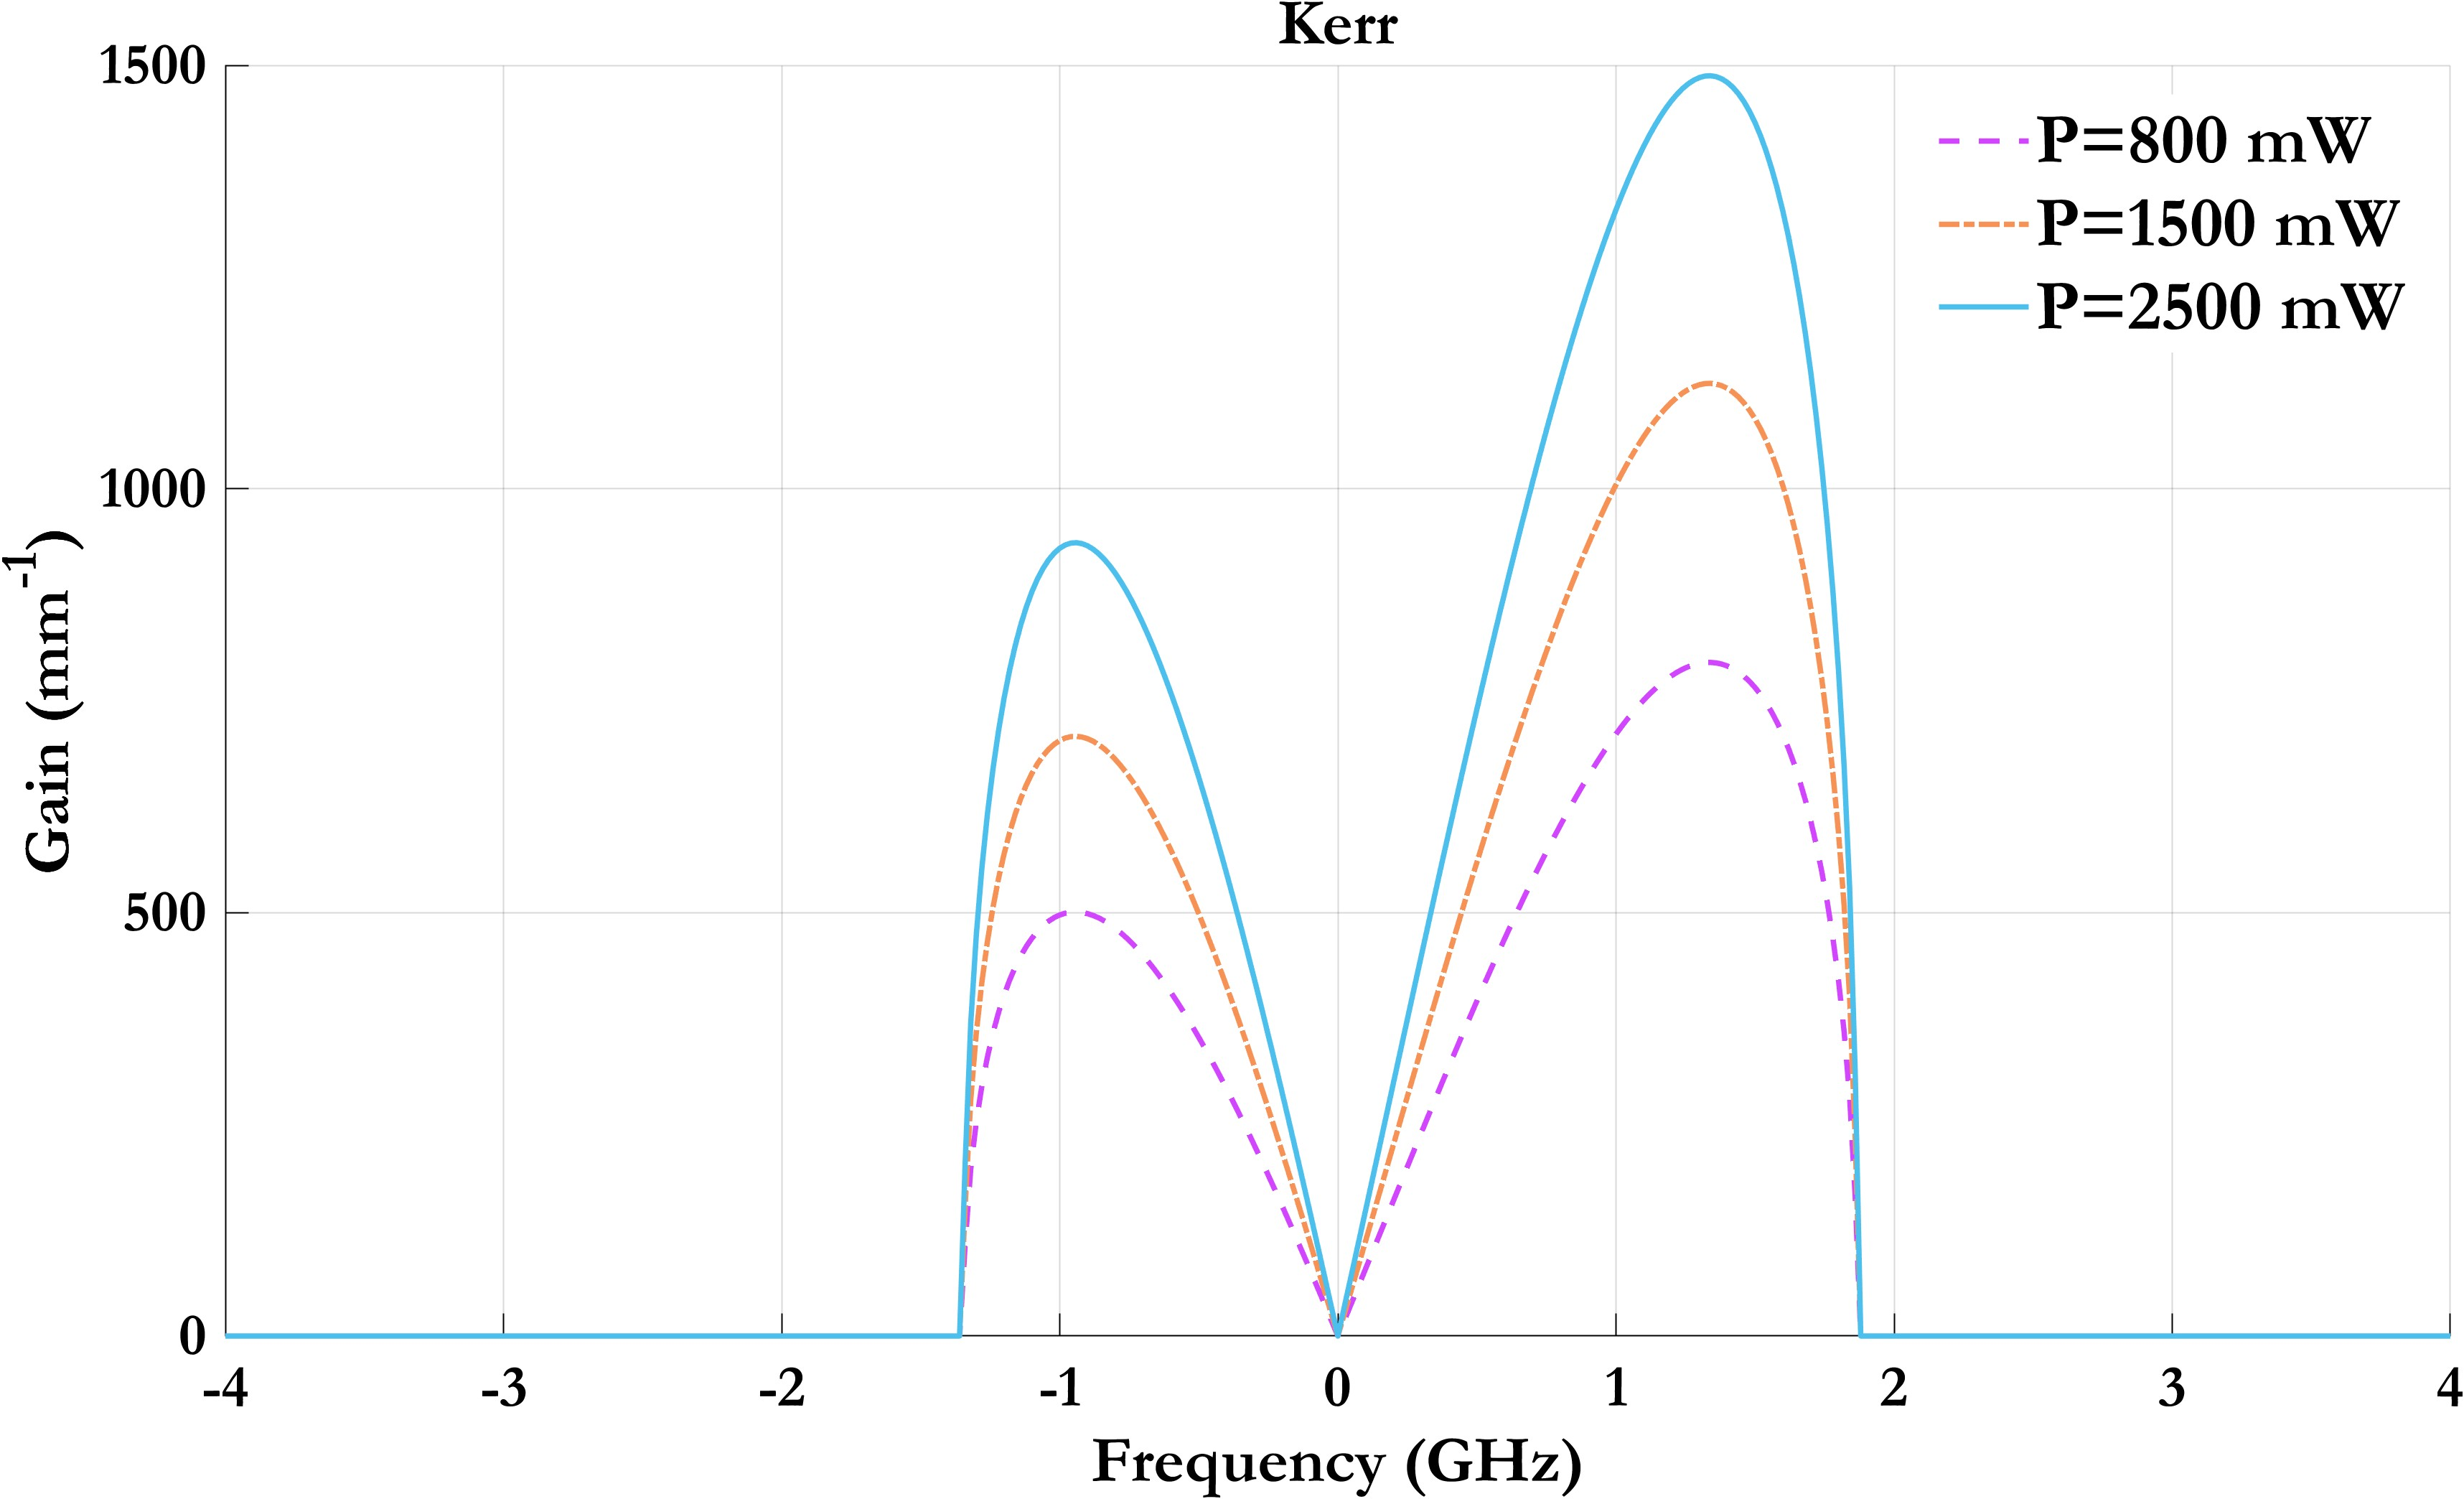
\includegraphics[width=0.7\linewidth]{Plots/G_v_Power.jpeg}
    \caption{Gain vs Frequency for $4^{th}$ order dispersion}
    \label{fig:G_v_P}
\end{figure}
This plot illustrates the \textit{modulation instability}~\cite{lighthall} (MI) gain as a function of frequency detuning in a semiconductor quantum dot medium governed by Kerr nonlinearity, under varying continuous-wave (CW) pump powers. The gain \( G \), expressed in ${mm^{-1}}$, is plotted against the frequency detuning \( \Omega \) (in ${GHz}$) for three distinct pump powers: ${800}{mW}$ (magenta dashed), ${1500}{mW}$ (orange dash-dotted), and ${2500}{mW}$ (cyan solid).

At all power levels, MI sidebands are symmetrically distributed about the central frequency (\( \Omega = 0 \)), indicating a phase-matched four-wave mixing (FWM) process. As the pump power increases, both the gain bandwidth and peak gain rise significantly, attributed to enhanced self-phase modulation (SPM) arising from a higher nonlinear refractive index \( n_2 \). For instance, at ${800}{mW}$, the gain peaks near ${700}{mm^{-1}}$ at \( \Omega \approx \pm {1.2}{GHz} \), whereas at ${2500}{mW}$, the peak exceeds ${1400}{mm^{-1}}$ with sidebands shifting to \( \Omega \approx \pm {1.9}{GHz} \).

The parabolic gain profiles emerge from the interplay between Kerr-induced phase modulation and higher-order dispersion, dominated by the fourth-order dispersion term \( \beta_4 \). The gain drops to zero at \( \Omega = 0 \), consistent with the phase mismatch criterion for MI.

Such gain spectra are pivotal in applications such as ultrafast pulse generation, optical frequency combs, and spontaneous MI-driven supercontinuum generation. The power dependence provides tunability, making quantum-dot-based platforms highly attractive for nonlinear integrated photonics.

Here we did the waterfall plot of Kerr using $2^{nd}$ and \(4^{th}\) order dispersion. 

\begin{figure}[h]
  \centering
  \begin{minipage}{0.48\textwidth}
    \centering
    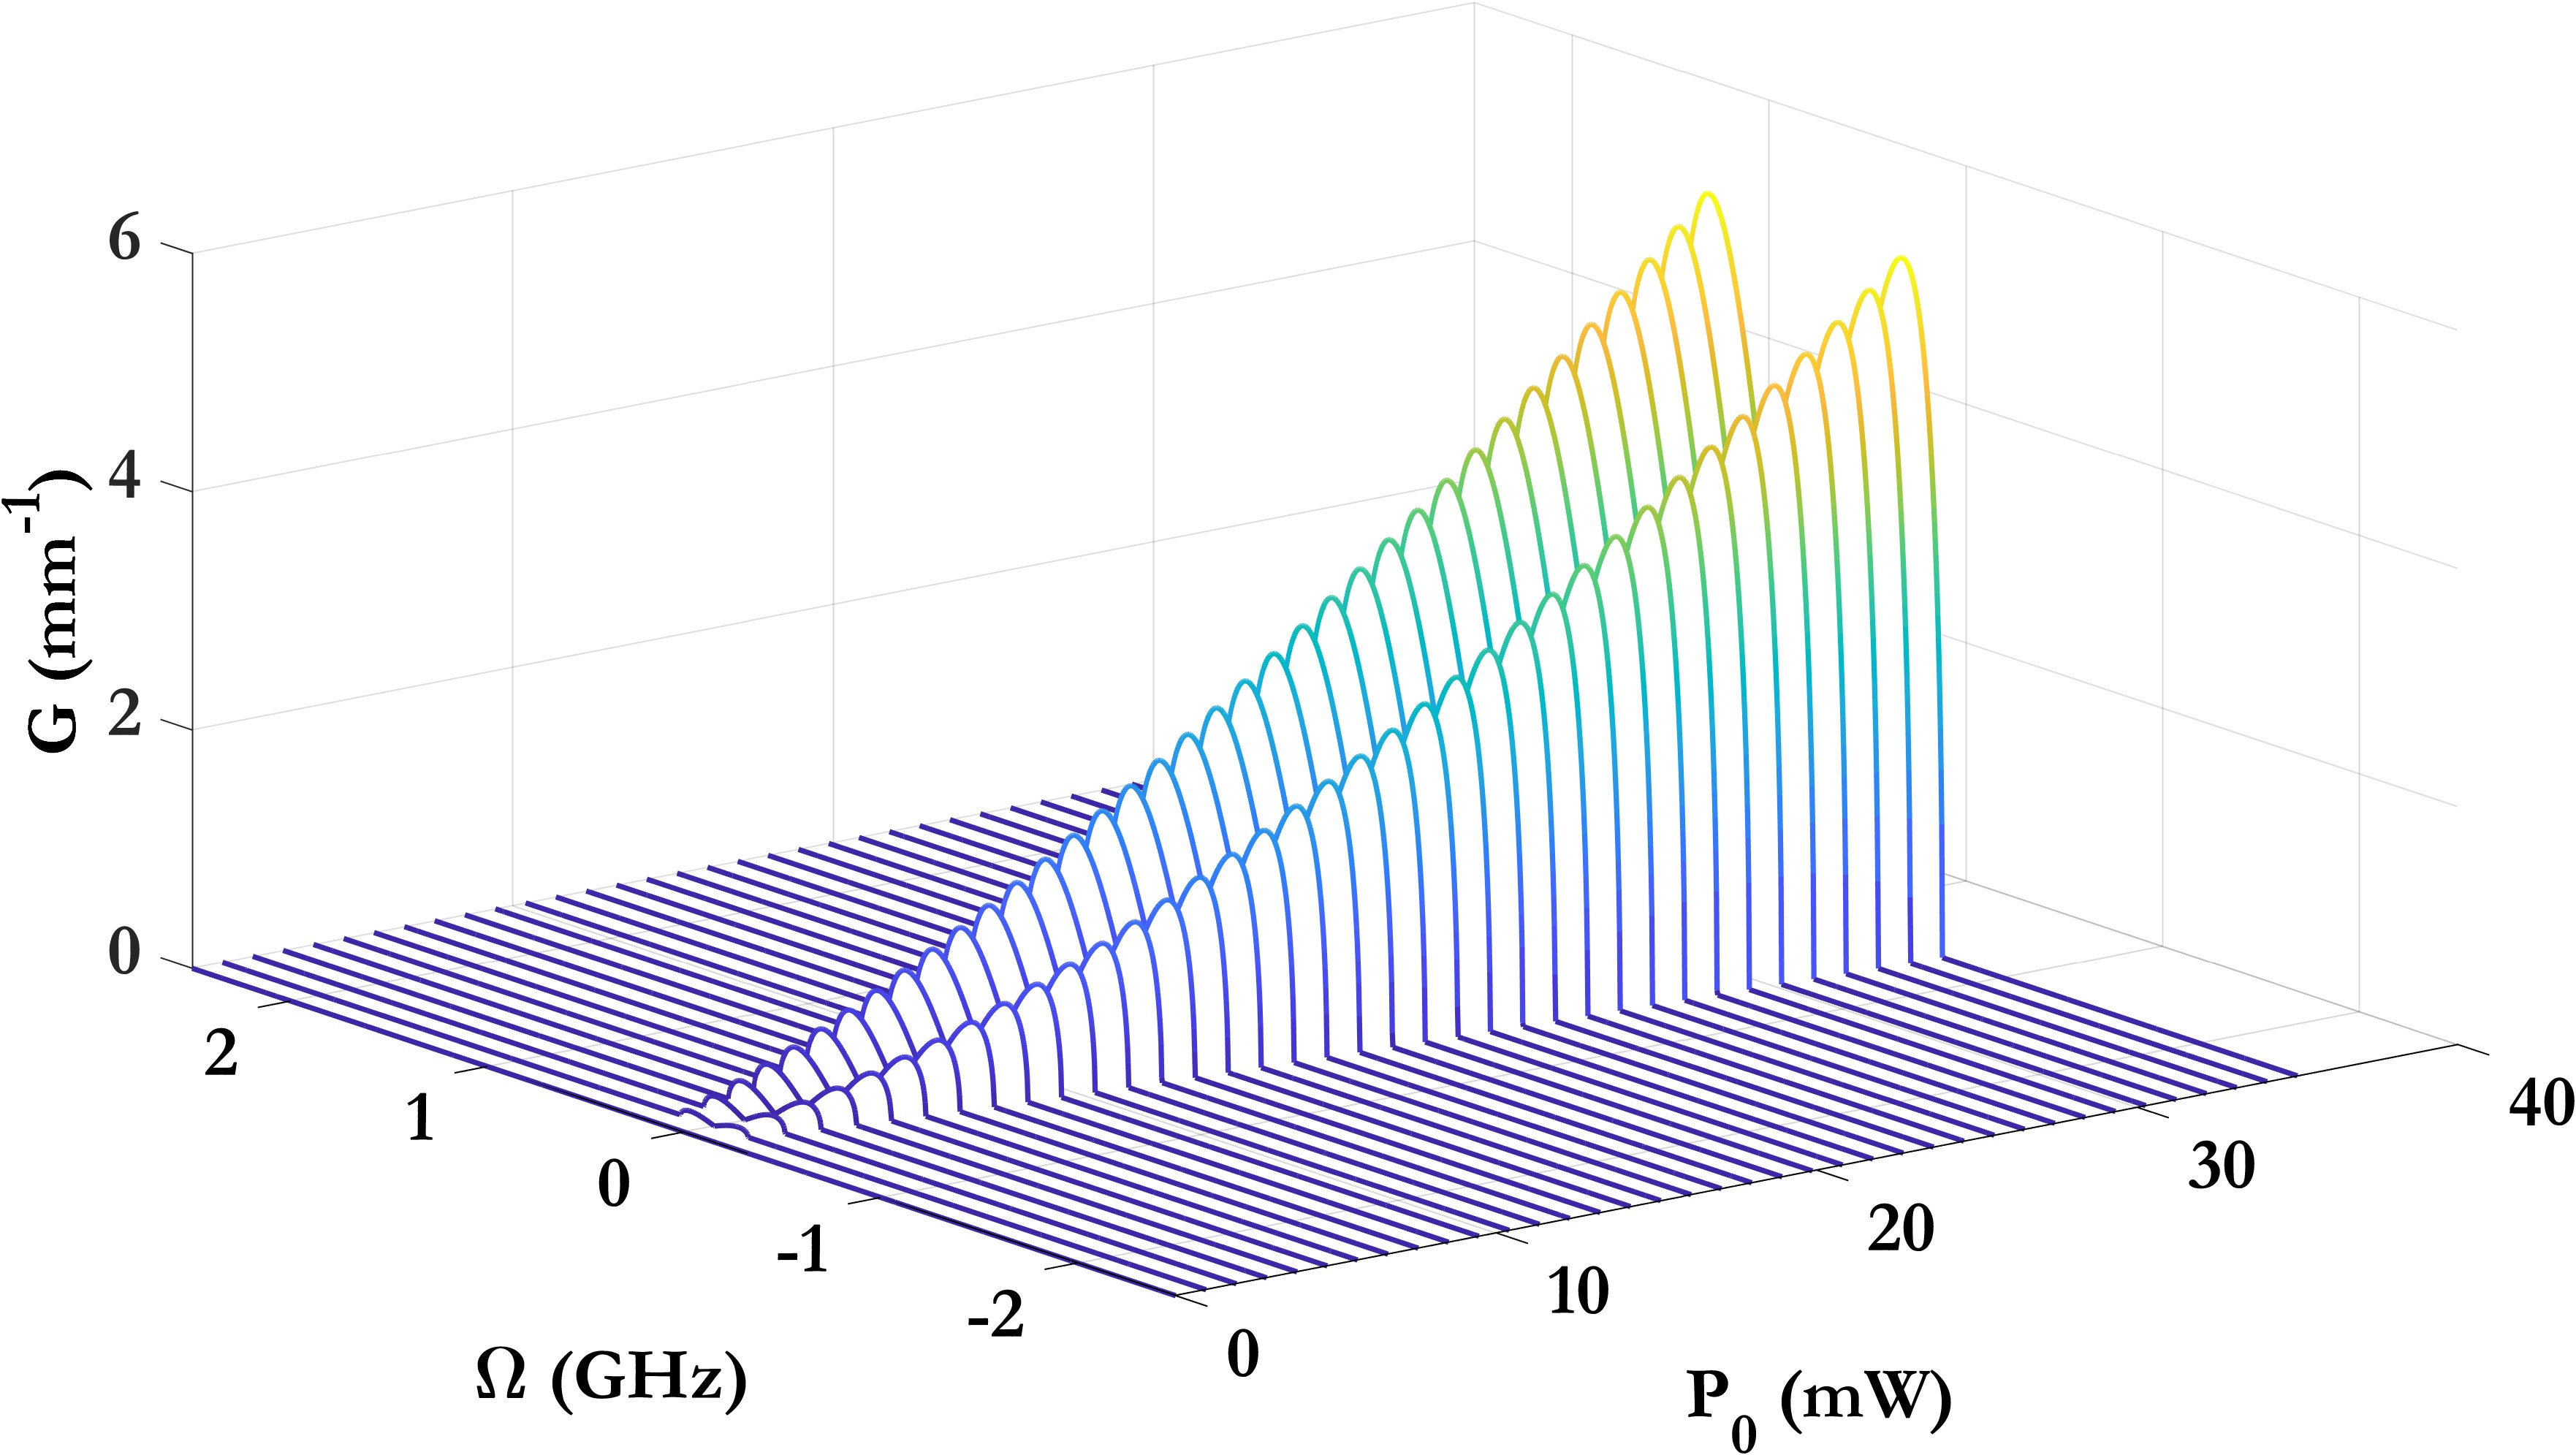
\includegraphics[width=\linewidth]{Plots/Beta2_Kerr.jpeg}
    \subcaption{}
  \end{minipage}%
  \hfill
  \begin{minipage}{0.48\textwidth}
    \centering
    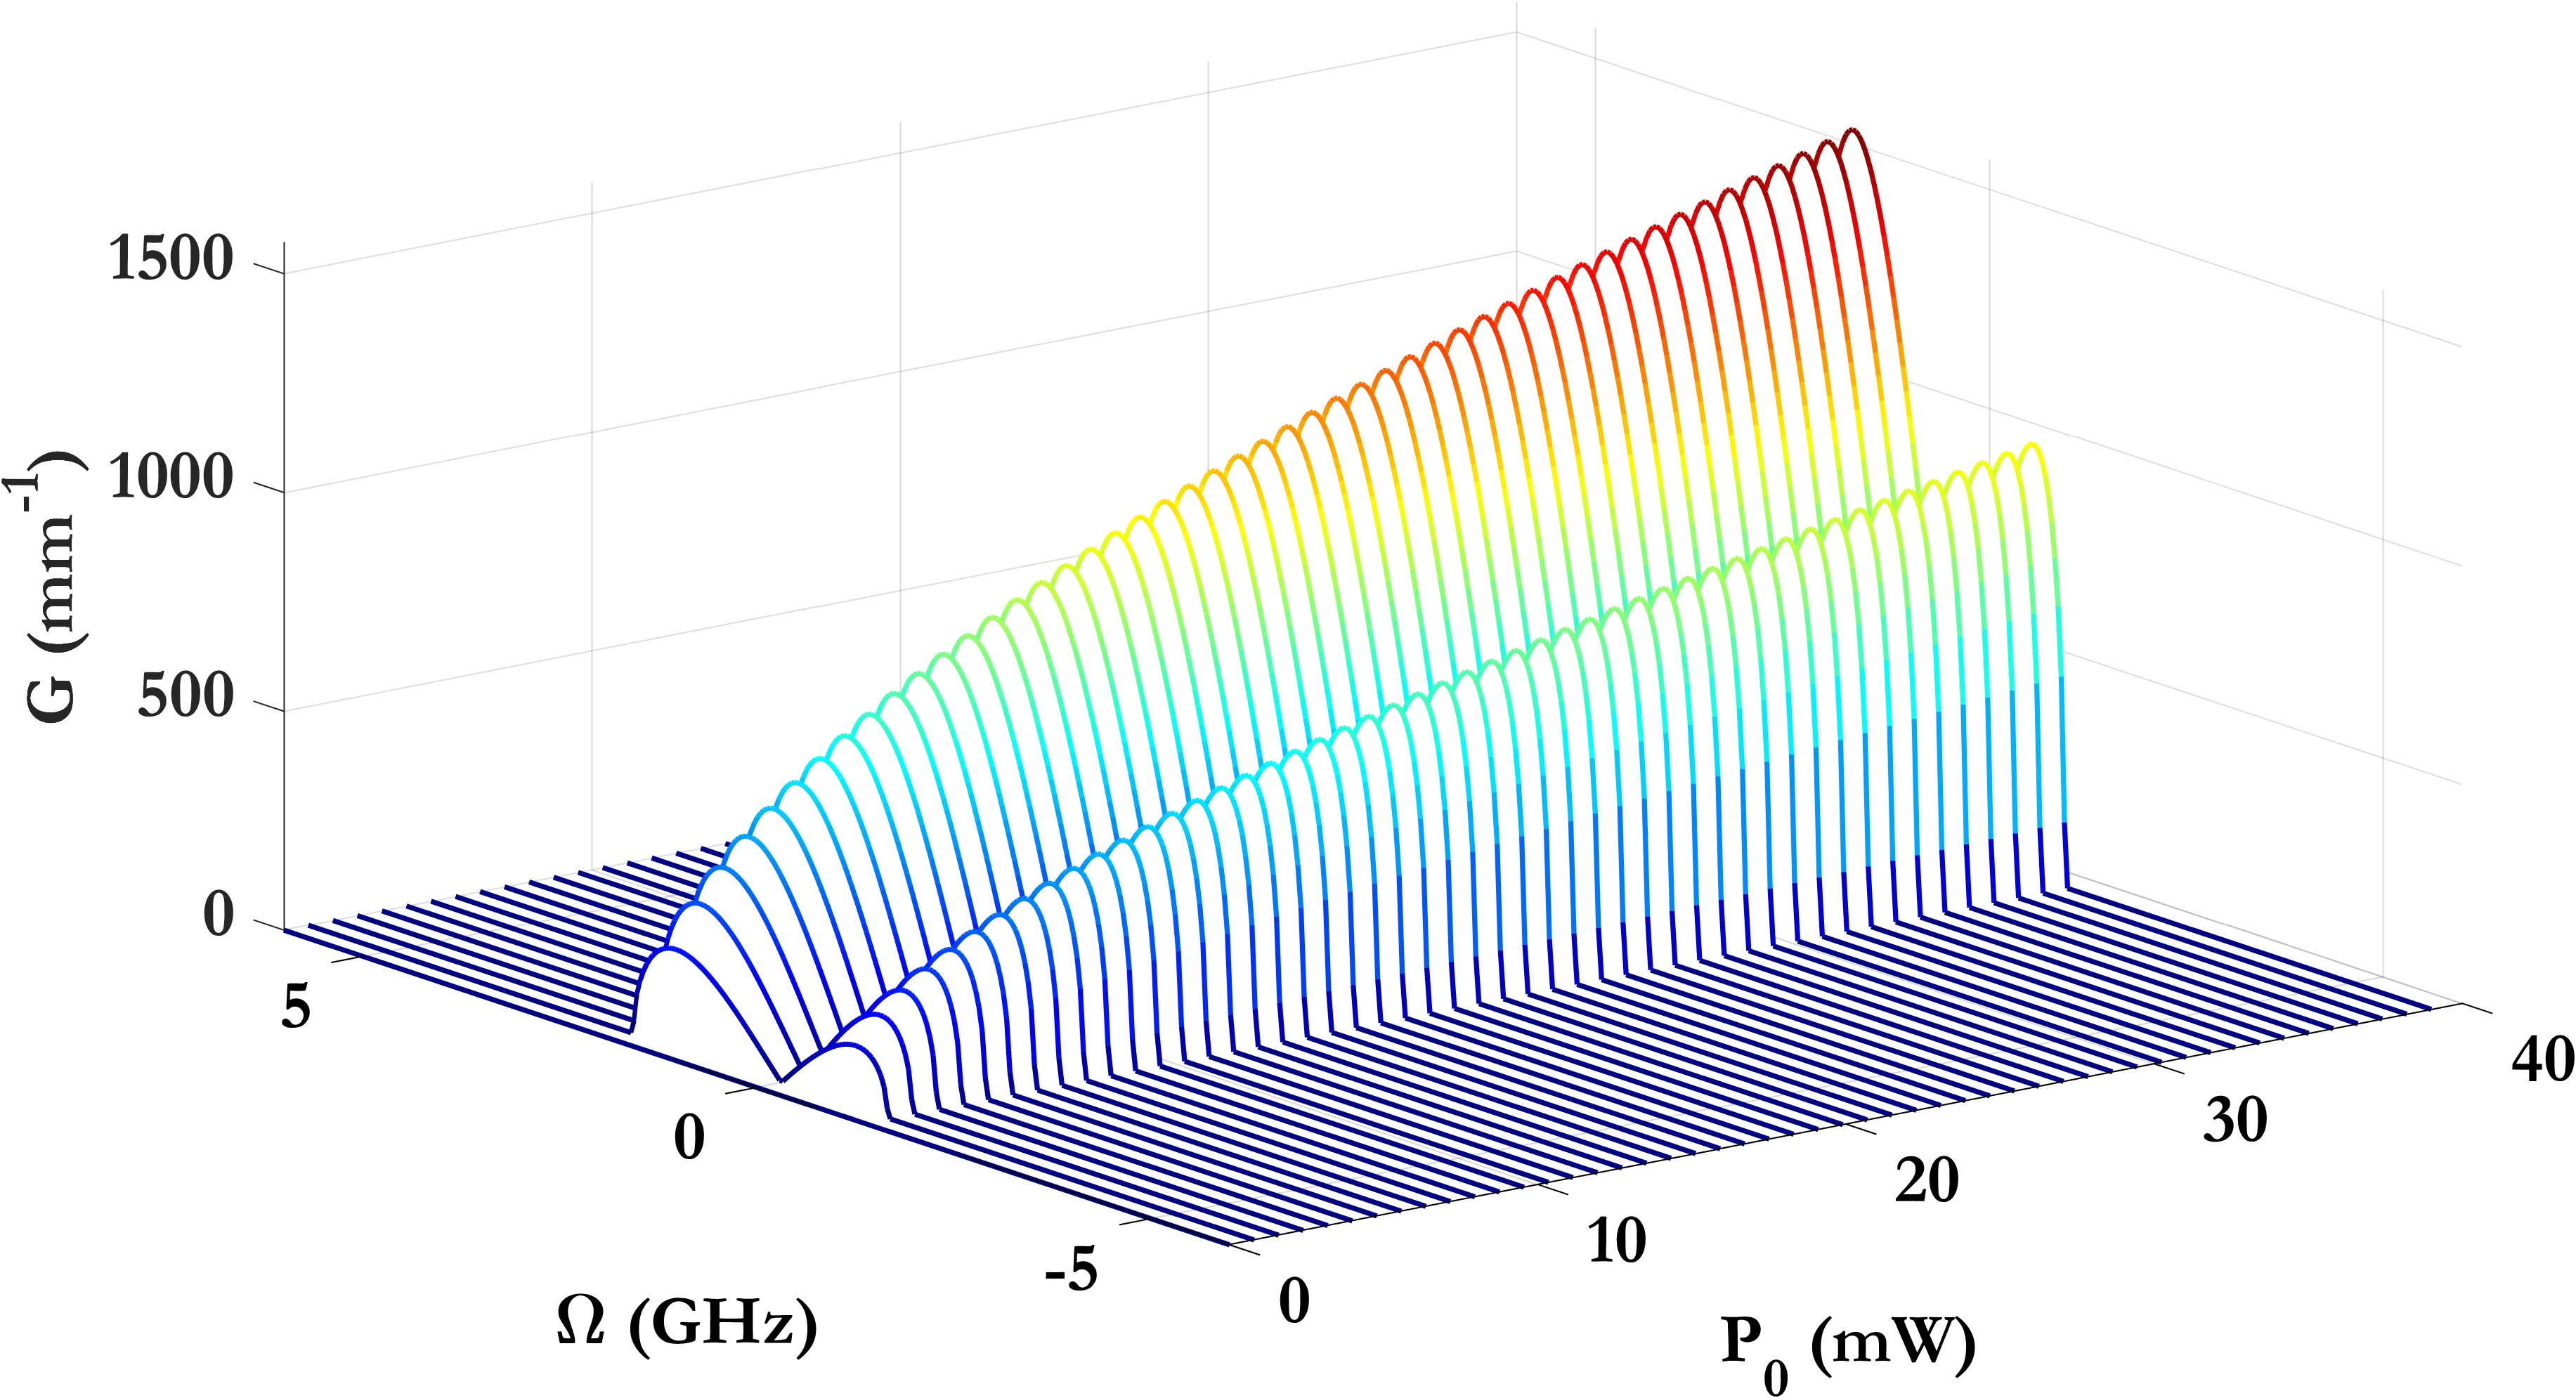
\includegraphics[width=\linewidth]{Plots/Beta4_Kerr.jpeg}
    \subcaption{}
  \end{minipage}
  \caption{Variation of MI gain with the frequency and power in absence and presence of $4^{th}$ order dispersion (i.e., $\beta_4=0$). (a) In absence of $\beta_4$, only Kerr nonlinearity present. (b) In presence of $\beta_4$, only Kerr nonlinearity present.}
  \label{fig:waterfall}
 \end{figure}
This 3D plot characterizes the Modulation Instability~\cite{lighthall} (MI) gain spectrum \( G(\Omega, P_0) \) in semiconductor quantum dots, revealing the conditions under which small perturbations on a continuous wave grow exponentially due to the nonlinear interplay between the Kerr effect and group velocity dispersion (GVD). The vertical axis represents the MI gain in ${mm^{-1}}$, while the horizontal axes denote the angular frequency detuning \( \Omega \) (in ${GHz}$) and the input continuous-wave optical power \( P_0 \) (in ${mW}$).

The MI gain is negligible at low power levels, but a distinct threshold appears near \( P_0 \approx 5 \, {mW} \), beyond which the gain rises sharply, indicative of a phase-matched four-wave mixing process driven by cubic (\( \chi^{(3)} \)) nonlinearity. The peak gain approaches approximately \( G \approx 6 \, {mm^{-1}} \) at \( P_0 \approx 35 \, {mW} \), centered around \( \Omega \approx \pm 1.2 \, {GHz} \). The symmetric spectral broadening with respect to zero detuning indicates a balanced sideband amplification mechanism.

For the \(4^{th}\) order dispersion we can see The MI bands span up to $\pm5GHz$, and the gain profile becomes more structured due to the higher-order phase mismatch. These features are crucial for tailoring spectral shaping, generating ultra-broadband combs, and enhancing pulse breakup dynamics in QD-based nonlinear photonic platforms.

Such characteristics make QD systems prime candidates for tunable broadband sources, soliton generation, and high-speed optical signal processing.
\newpage

\section{Conclusion}
In summary we have examined dispersive and optical nonlinear properties of SQDs under the regime of electromagnetic induced transparency. The magnitude of this nonlinearity could be controlled by controlling the Rabi frequency and detuning of the con- trolling fields. The intensity and the width of modulation spectra could be controlled by two control fields. A propagating continuous wave or quasi continuous probe beam undergoes modulation instability~\cite{lighthall} owing to the presence of large nonlinearity. The growth of instability and bandwidth of unstable frequencies could be externally govern by the Rabi frequency, two control detunings and power of the probe beam. Both fourth order dispersion and quintic nonlinearity reduce the growth and bandwidth of the unstable frequency.

\newpage
\section*{Acknowledgment}
My sincerest gratitude to everyone who supported me throughout the endeavour of developing the project. First, I thanks to My supervisor of this Project Dr.Rohit Mukherjee for his invaluable guidance, encouragement, and his feedback, which is a vital role to make the direction and success of this work. I am also grateful to Our HOD of Department of Physics of RKMVCC Dr.Ashoke Kumar Paul for providing me the necessary resources and a a very needful environment to undertake this project.

\newpage
\bibliographystyle{unsrtnat}
\bibliography{citations}
\end{document}